\documentclass[a4paper, 12pt]{scrartcl}
\usepackage[ngerman]{babel}
\usepackage[utf8]{inputenc}
\usepackage[T1]{fontenc}
\usepackage{lmodern}

\usepackage{graphicx}
\usepackage{amssymb}
\usepackage{hyperref}
\usepackage{float}
\usepackage{enumitem}
\usepackage{wrapfig}
\usepackage{units}
\usepackage{mathtools}
\usepackage{ziffer}
\usepackage{subcaption}
\usepackage{listings}
\usepackage{color}

\usepackage{geometry}
\geometry{a4paper, top=20mm, left=20mm, right=20mm, bottom=20mm, headsep=10mm, footskip=10mm}
\linespread{1.2}
\setitemize{leftmargin=*}
\parindent0cm
	
\lstset{literate=%
	{Ö}{{\"O}}1
	{Ä}{{\"A}}1
	{Ü}{{\"U}}1
	{ü}{{\"u}}1
	{ä}{{\"a}}1
	{ö}{{\"o}}1
	{█}{{$\blacksquare$}}1
	{~}{{\textasciitilde}}1
}

\definecolor{mygreen}{rgb}{0,0.6,0}
\definecolor{mygray}{rgb}{0.5,0.5,0.5}
\definecolor{mymauve}{rgb}{0.58,0,0.82}
\definecolor{deepred}{rgb}{0.6,0,0}

\lstset{ %
	backgroundcolor=\color{white},   % choose the background color; you must add \usepackage{color} or \usepackage{xcolor}; should come as last argument
	basicstyle=\ttfamily\scriptsize,          % the size of the fonts that are used for the code
	breakatwhitespace=false,         % sets if automatic breaks should only happen at whitespace
	breaklines=true,                 % sets automatic line breaking
	captionpos=b,                    % sets the caption-position to bottom
	commentstyle=\color{mygreen},    % comment style
	deletekeywords={...},            % if you want to delete keywords from the given language
	escapeinside={\%*}{*)},          % if you want to add LaTeX within your code
	extendedchars=true,              % lets you use non-ASCII characters; for 8-bits encodings only, does not work with UTF-8
	frame=single,	                 % adds a frame around the code
	keepspaces=true,                 % keeps spaces in text, useful for keeping indentation of code (possibly needs columns=flexible)
	keywordstyle=\color{blue},       % keyword style
	language=Python,                 % the language of the code
	morekeywords={*,...},            % if you want to add more keywords to the set
	emph={makevideo,checkgreen,checkblue,lenken,line,linienfahren,main},
	emphstyle=\color{deepred},
	numbers=left,                    % where to put the line-numbers; possible values are (none, left, right)
	numbersep=5pt,                   % how far the line-numbers are from the code
	numberstyle=\tiny\color{mygray}, % the style that is used for the line-numbers
	rulecolor=\color{black},         % if not set, the frame-color may be changed on line-breaks within not-black text (e.g. comments (green here))
	showspaces=false,                % show spaces everywhere adding particular underscores; it overrides 'showstringspaces'
	showstringspaces=false,          % underline spaces within strings only
	showtabs=false,                  % show tabs within strings adding particular underscores
	stepnumber=2,                    % the step between two line-numbers. If it's 1, each line will be numbered
	stringstyle=\color{mymauve},     % string literal style
	tabsize=2,	                     % sets default tabsize to 2 spaces
	title=\lstname                   % show the filename of files included with \lstinputlisting; also try caption instead of title
}
 
\begin{document}
\thispagestyle{empty}

\begin{flushright}
	
\includegraphics[width=5cm]{HAW_Logo.eps}
\end{flushright}

Hochschule für Angewandte Wissenschaften Hamburg\\
Fakultät Design, Medien und Information\\
Department Medientechnik\\[1ex]
IT-Systeme\\
Prof. Dr. Torsten Edeler

\vspace{1cm}

\begin{center}
	\large{Projektbericht}\\
	\LARGE{Raspberry Car --- Racingteam II}	
	\vspace{2ex}
	
	\large{
		Jörn Kogerup, 2248604\\
		Darius Weiberg, 2144123\\
		Mirco Hülsemann, 2248464
	}
	\vspace{2ex}
	
	\large{20. Februar 2018}
\end{center}

\vspace{1cm}

\begin{figure}[H] 
	\centering
	\makebox[\textwidth]{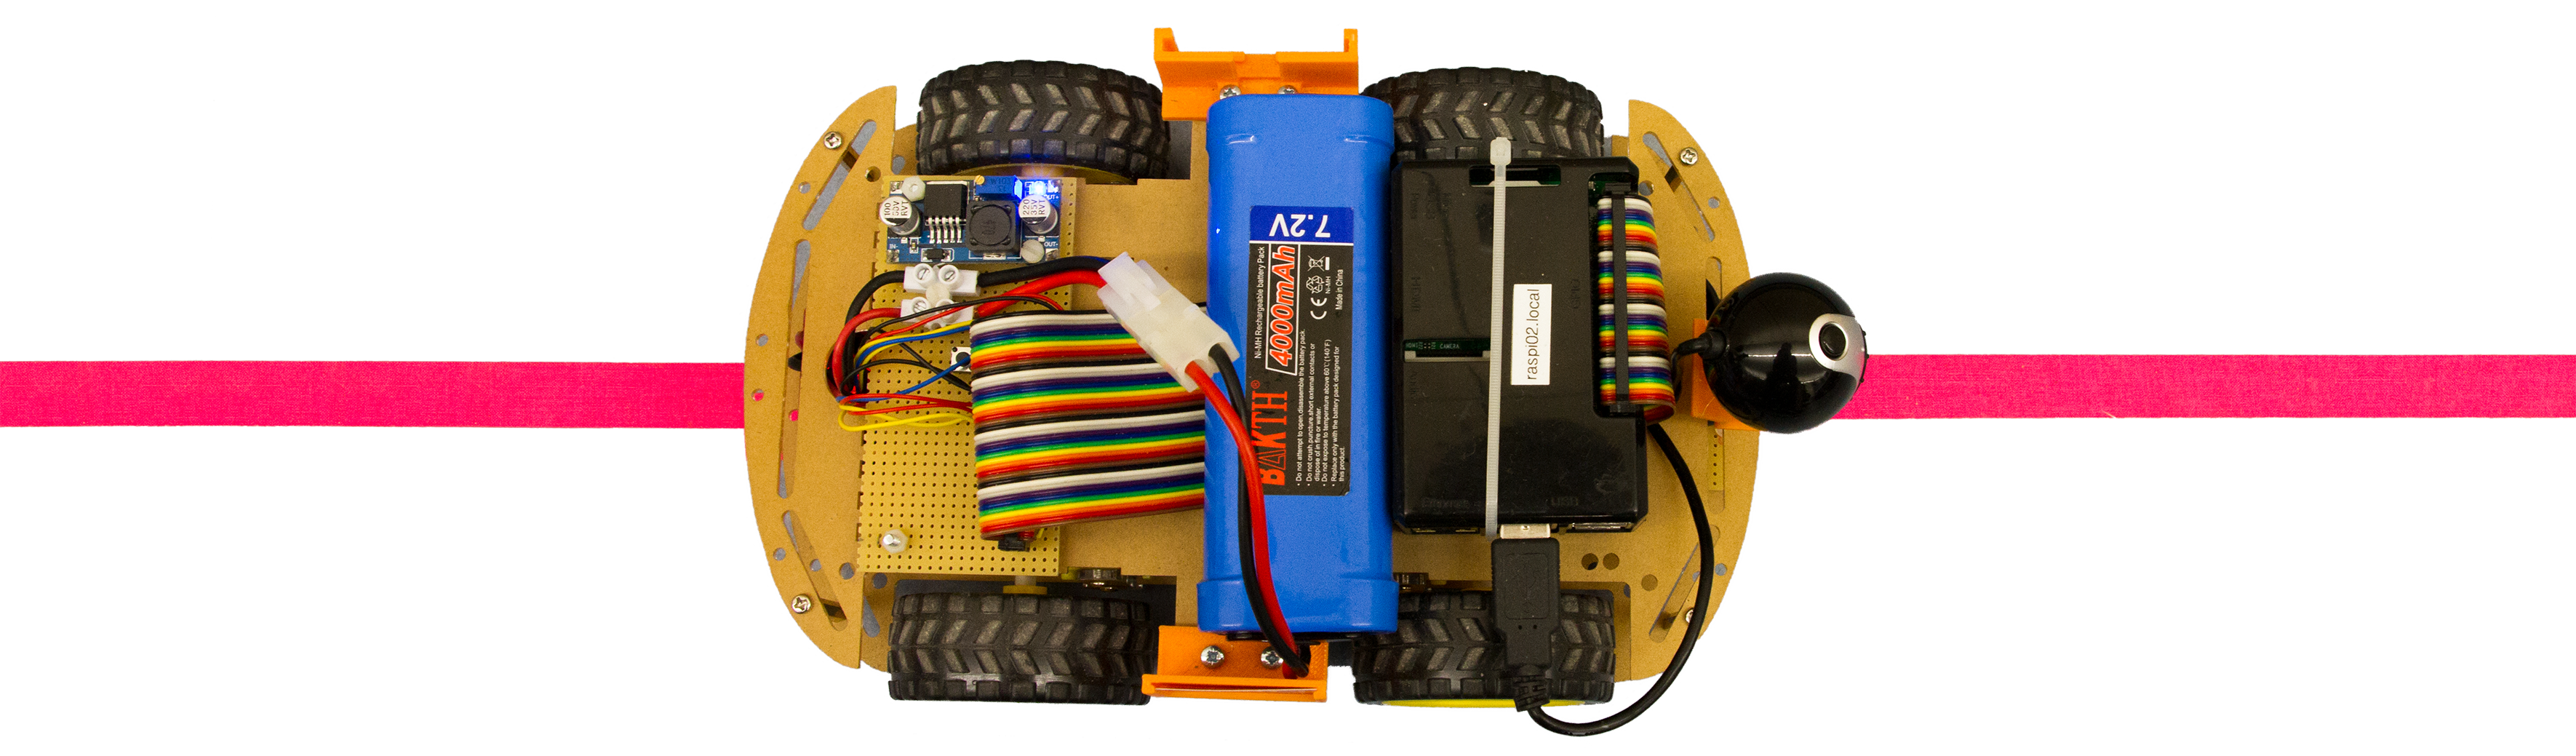
\includegraphics[width=\paperwidth]{Titel.png}}
	\caption{Auto von oben}
\end{figure}

\newpage

\tableofcontents

\newpage

\section{Einleitung}

Dieser Projektbericht dient der Dokumentation des Projekts „Entwicklung eines selbstfahrenden Autos“ im Modul IT-Systeme des Studiengangs Medientechnik an der HAW Hamburg im Wintersemester 2017/18.

Autonomes Fahren ist derzeit ein großes und hochaktuelles Forschungsthema vieler Universitäten, IT-Unternehmen und Automobilhersteller. Mit Hochdruck arbeiten Unternehmen wie Tesla, General Motors oder Waymo zusammen mit IT-Firmen wie Intel und Google daran, selbstfahrende Autos für die breite Masse verfügbar zu machen.

Aufgrund der aktuellen Relevanz und der Tatsache, dass ein selbstfahrendes Auto die ideale Verkörperung eines informationstechnischen Systems ist, wurde dieses Thema als Projekt für die Veranstaltung „IT-Systeme“ im Wintersemester 2017/2018 auserwählt.

Der vorliegende Abschlussbericht enthält Erläuterungen zum Projektziel, Projektumfeld sowie zu den gegebenen technischen Rahmenbedingungen. Es werden die einzelnen Schritte des Entwicklungsprozesses dokumentiert und Probleme genannt, die während der Entwicklung auftraten. Der Bericht endet mit einer Erörterung über die möglichen Weiterentwicklungen des Projekts.

\section{Konzept}

\subsection{Projektvorstellung}

Im Rahmen der Vorlesung IT-Systeme (5. Semester des Studiengangs Medientechnik) sollen die Studierenden in kleinen Gruppen ein autonomes Modellbau-Auto entwickeln, welches in der Lage sein soll, mithilfe von Sensoren und Kamera selbstständig eine vorher definierte Rennstrecke abzufahren. Die Aufgaben der Studierenden umfassen dabei:

\begin{itemize}
	\item eine konzeptionelle Planung zur Umsetzung des Projekts,
	\item die Konstruktion des Modellbau-Autos (dabei wird ein Bausatz verwendet) sowie der Rennstrecke,
	\item die Auseinandersetzung mit der Funktionsweise der elektrischen Komponenten,
	\item die Verschaltung der elektrischen Komponenten,
	\item Programmierung und Implementierung des Steuer-Codes auf einem Raspberry Pi.
\end{itemize}

Als zeitlicher Rahmen ist ein Semester vorgesehen. Pro Woche gibt es eine dreistündige Einheit, in der die Studierenden unter Betreuung am Projekt arbeiten können. Es ist jedoch auch möglich, außerhalb dieser Einheit mit dem Projekt fortzuführen.

Es gibt zudem zwei Challenge-Termine im Semester, zu denen bestimmte Zwischenziele erreicht werden müssen. Auf diese Art wird das Vorankommen des Projekts überprüft und gewährleistet. Am Ende des Semesters erfolgt eine Generalprobe und schließlich die Projektausstellung.

\subsection{Projektziel}

Ziel des Projekts ist es, ein autonomes Auto zu entwickeln, welches mithilfe von Mikrocomputer, Kamera und Abstandssensoren zwei Runden auf einer definierten Rennstrecke selbstständig und erfolgreich absolviert. Dabei sollen die Autos einzeln starten, es befindet sich also nie mehr als ein Auto auf der Strecke. Die Gruppe, deren Auto den Kurs am schnellsten durchfährt, wird als Gewinner geehrt.

Auf dem Weg zu diesem Ziel gibt es im Laufe des Semesters zudem zwei Zwischenziele, sogenannte Challenges, die erfolgreich absolviert werden müssen. Das erste Zwischenziel ist eine Geradeausfahrt von 10 Metern mit Geschwindigkeitswechseln, das zweite Zwischenziel ist das Fahren entlang einer Wand mithilfe von Abstandssensoren.

\subsection{Die Rennstrecke}

\begin{wrapfigure}{L}[.5cm]{.33\textwidth}
	\centering
	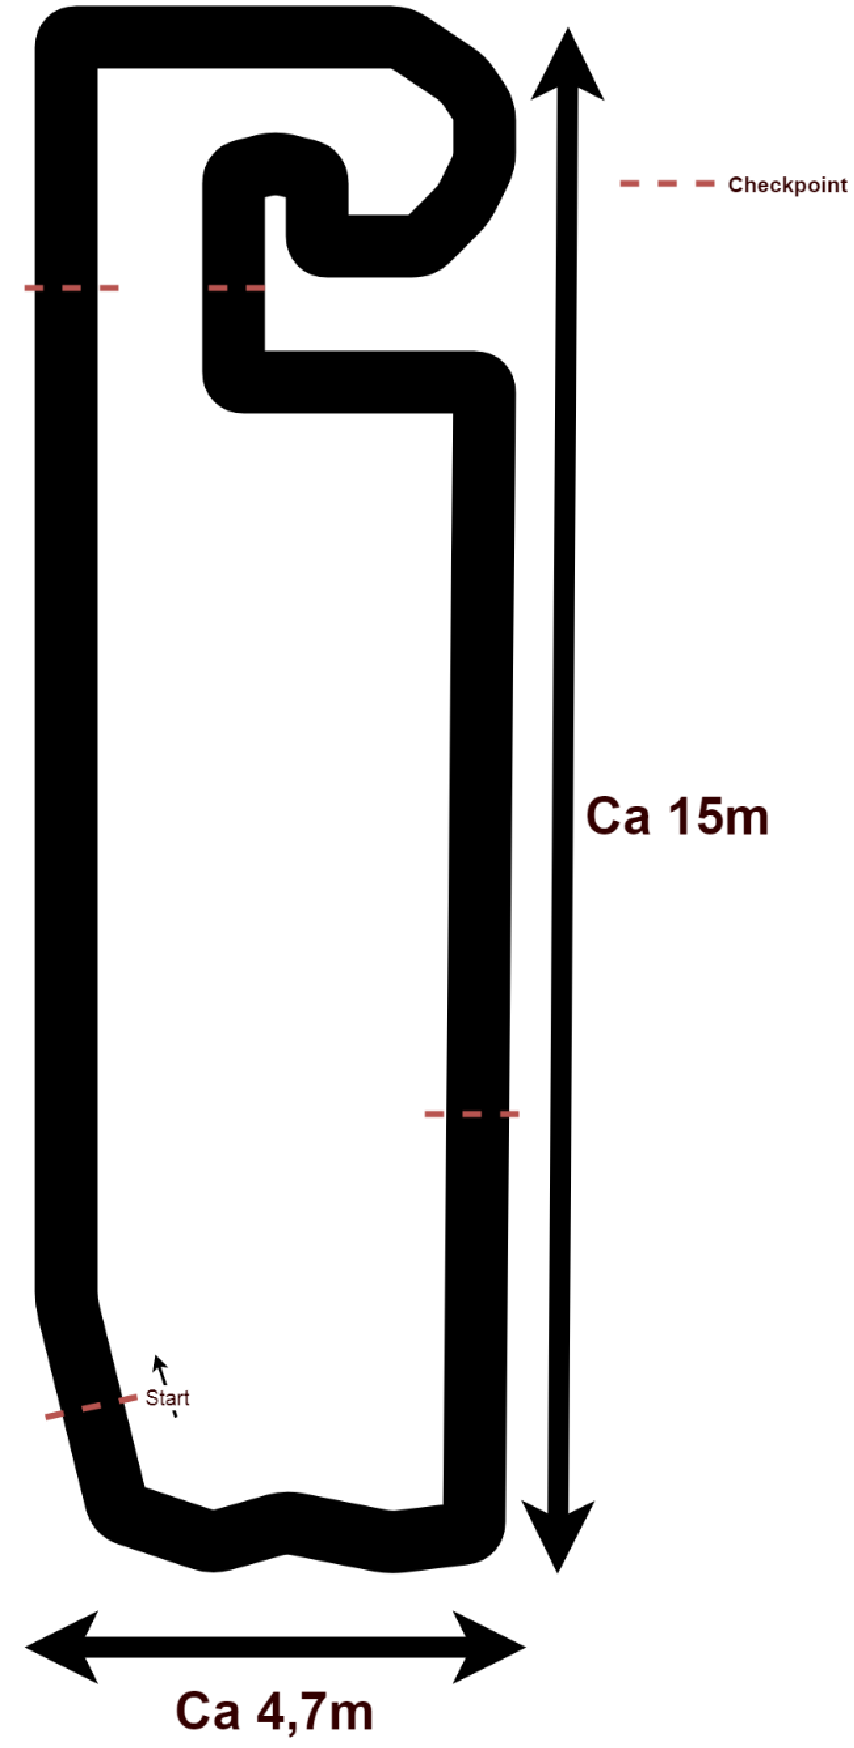
\includegraphics[width=.3\textwidth]{Rennstrecke.png}
	\caption{Rennstrecke}
	\label{rennstrecke}
\end{wrapfigure}

Die Rennstrecke, die es zu meistern gilt, wird am Anfang des Semesters grob definiert: Sie soll als geschlossene Rundstrecke (Startlinie = Ziellinie) in einem Laborraum der Hochschule aufgebaut werden. Im Wesentlichen soll sie aus einer Mittellinie sowie zwei Begrenzungslinien bestehen. Der Mittellinie gilt es zu folgen, die Begrenzungslinien dürfen nicht überschritten werden. Die Strecke soll außerdem mehrere Kurven mit verschiedenem Radius enthalten sowie einen geraden Abschnitt ohne Mittellinie entlang einer Wand. In diesem Abschnitt ohne Mittellinie sollen Abstandssensoren genutzt werden, um auf der Spur zu bleiben.

Die finale, endgültige Version der Rennstrecke wird im Laufe des Semesters anhand der oben genannten Richtlinien von einer Gruppe im Kurs entworfen und ist in nebenstehender Abbildung zu sehen.

Die Linien werden mit Klebeband realisiert, welches auf den Boden des Laborraums aufgeklebt wird. Als Mittellinie dient rotes Tape, als Begrenzungslinie schwarzes.

Aufgrund von Problemen mit den verfügbaren Abstandssensoren, die sich erst im Laufe des Semesters ergeben haben, ist der gerade Abschnitt entlang der Wand in der endgültigen Version auch mit einer Mittellinie versehen. Die Aufgabe, mithilfe von Abstandssensoren entlang einer Wand zu fahren, fällt somit -- zumindest in der Generalprobe und Projektausstellung -- weg.

Eine weitere Änderung der anfänglichen Version der Rennstrecke ist die Einführung einer Ampel an der Start- und Ziellinie. So sollen die Autos nur bei grünem Licht starten und automatisch anhalten, wenn das Licht blau geschaltet ist. Die Ampel wird durch einen LED-Streifen auf dem Boden realisiert.

\subsection{Das Auto}
Die Komponenten, die für den Bau des Autos verwendet werden dürfen, sind vorgegeben und werden von der Hochschule bereitgestellt:

\begin{itemize}
	\item Einfacher Modellbau-Auto-Bausatz, bestehend aus Rahmen, DC-Getriebemotoren und gummierten Rädern
	\item \unit[7,2]{V} NiMH-Akku mit einer Kapazität von \unit[4000]{mAh}
	\item Motortreiber L298N für DC-Motoren mit Dual-H-Bridge
	\item Raspberry Pi 3 Model B (4-Kern-CPU, \unit[1,2]{GHz}, \unit[1]{GB} Ram, WLAN, Bluetooth)
	\item USB-Webcam ($640\times 480$ Pixel, \unit[30]{fps}, manueller Fokus)
	\item Ultraschallsensor HC-SR04 (messbare Distanz: \unit[2--300]{cm}, Auflösung: \unit[3]{mm}, max. 50 Messungen pro Sekunde)
\end{itemize}

Alle Komponenten (mit Ausnahme des Raspberry Pis) wurden im Hinblick auf einen möglichst günstigen Einkaufspreis ausgewählt. Dementsprechend sind die Erwartungen an Haltbarkeit, Genauigkeit und Ausfallsicherheit der Produkte und letztendlich an die Performance des Autos nicht allzu hoch.

Neben den aufgeführten Komponenten steht den Studierenden eine Werkstatt mit 3D-Drucker, Lötgerät und einer Vielzahl an Elektronikbauteilen (Kabel, Widerstände, Platinen \ldots) zur Verfügung.

Als Programmiersprache wird Python verwendet. Diese universelle Sprache zeichnet sich durch einfache und leicht verständliche Syntax, große Nutzerbasis sowie mächtige Bibliotheken aus und ist quasi Standardsprache auf dem Raspberry Pi.

\subsection{Konstruktion des Autos}

\begin{figure}[H] 
	\centering
	\begin{subfigure}{.5\textwidth} 
		\centering
		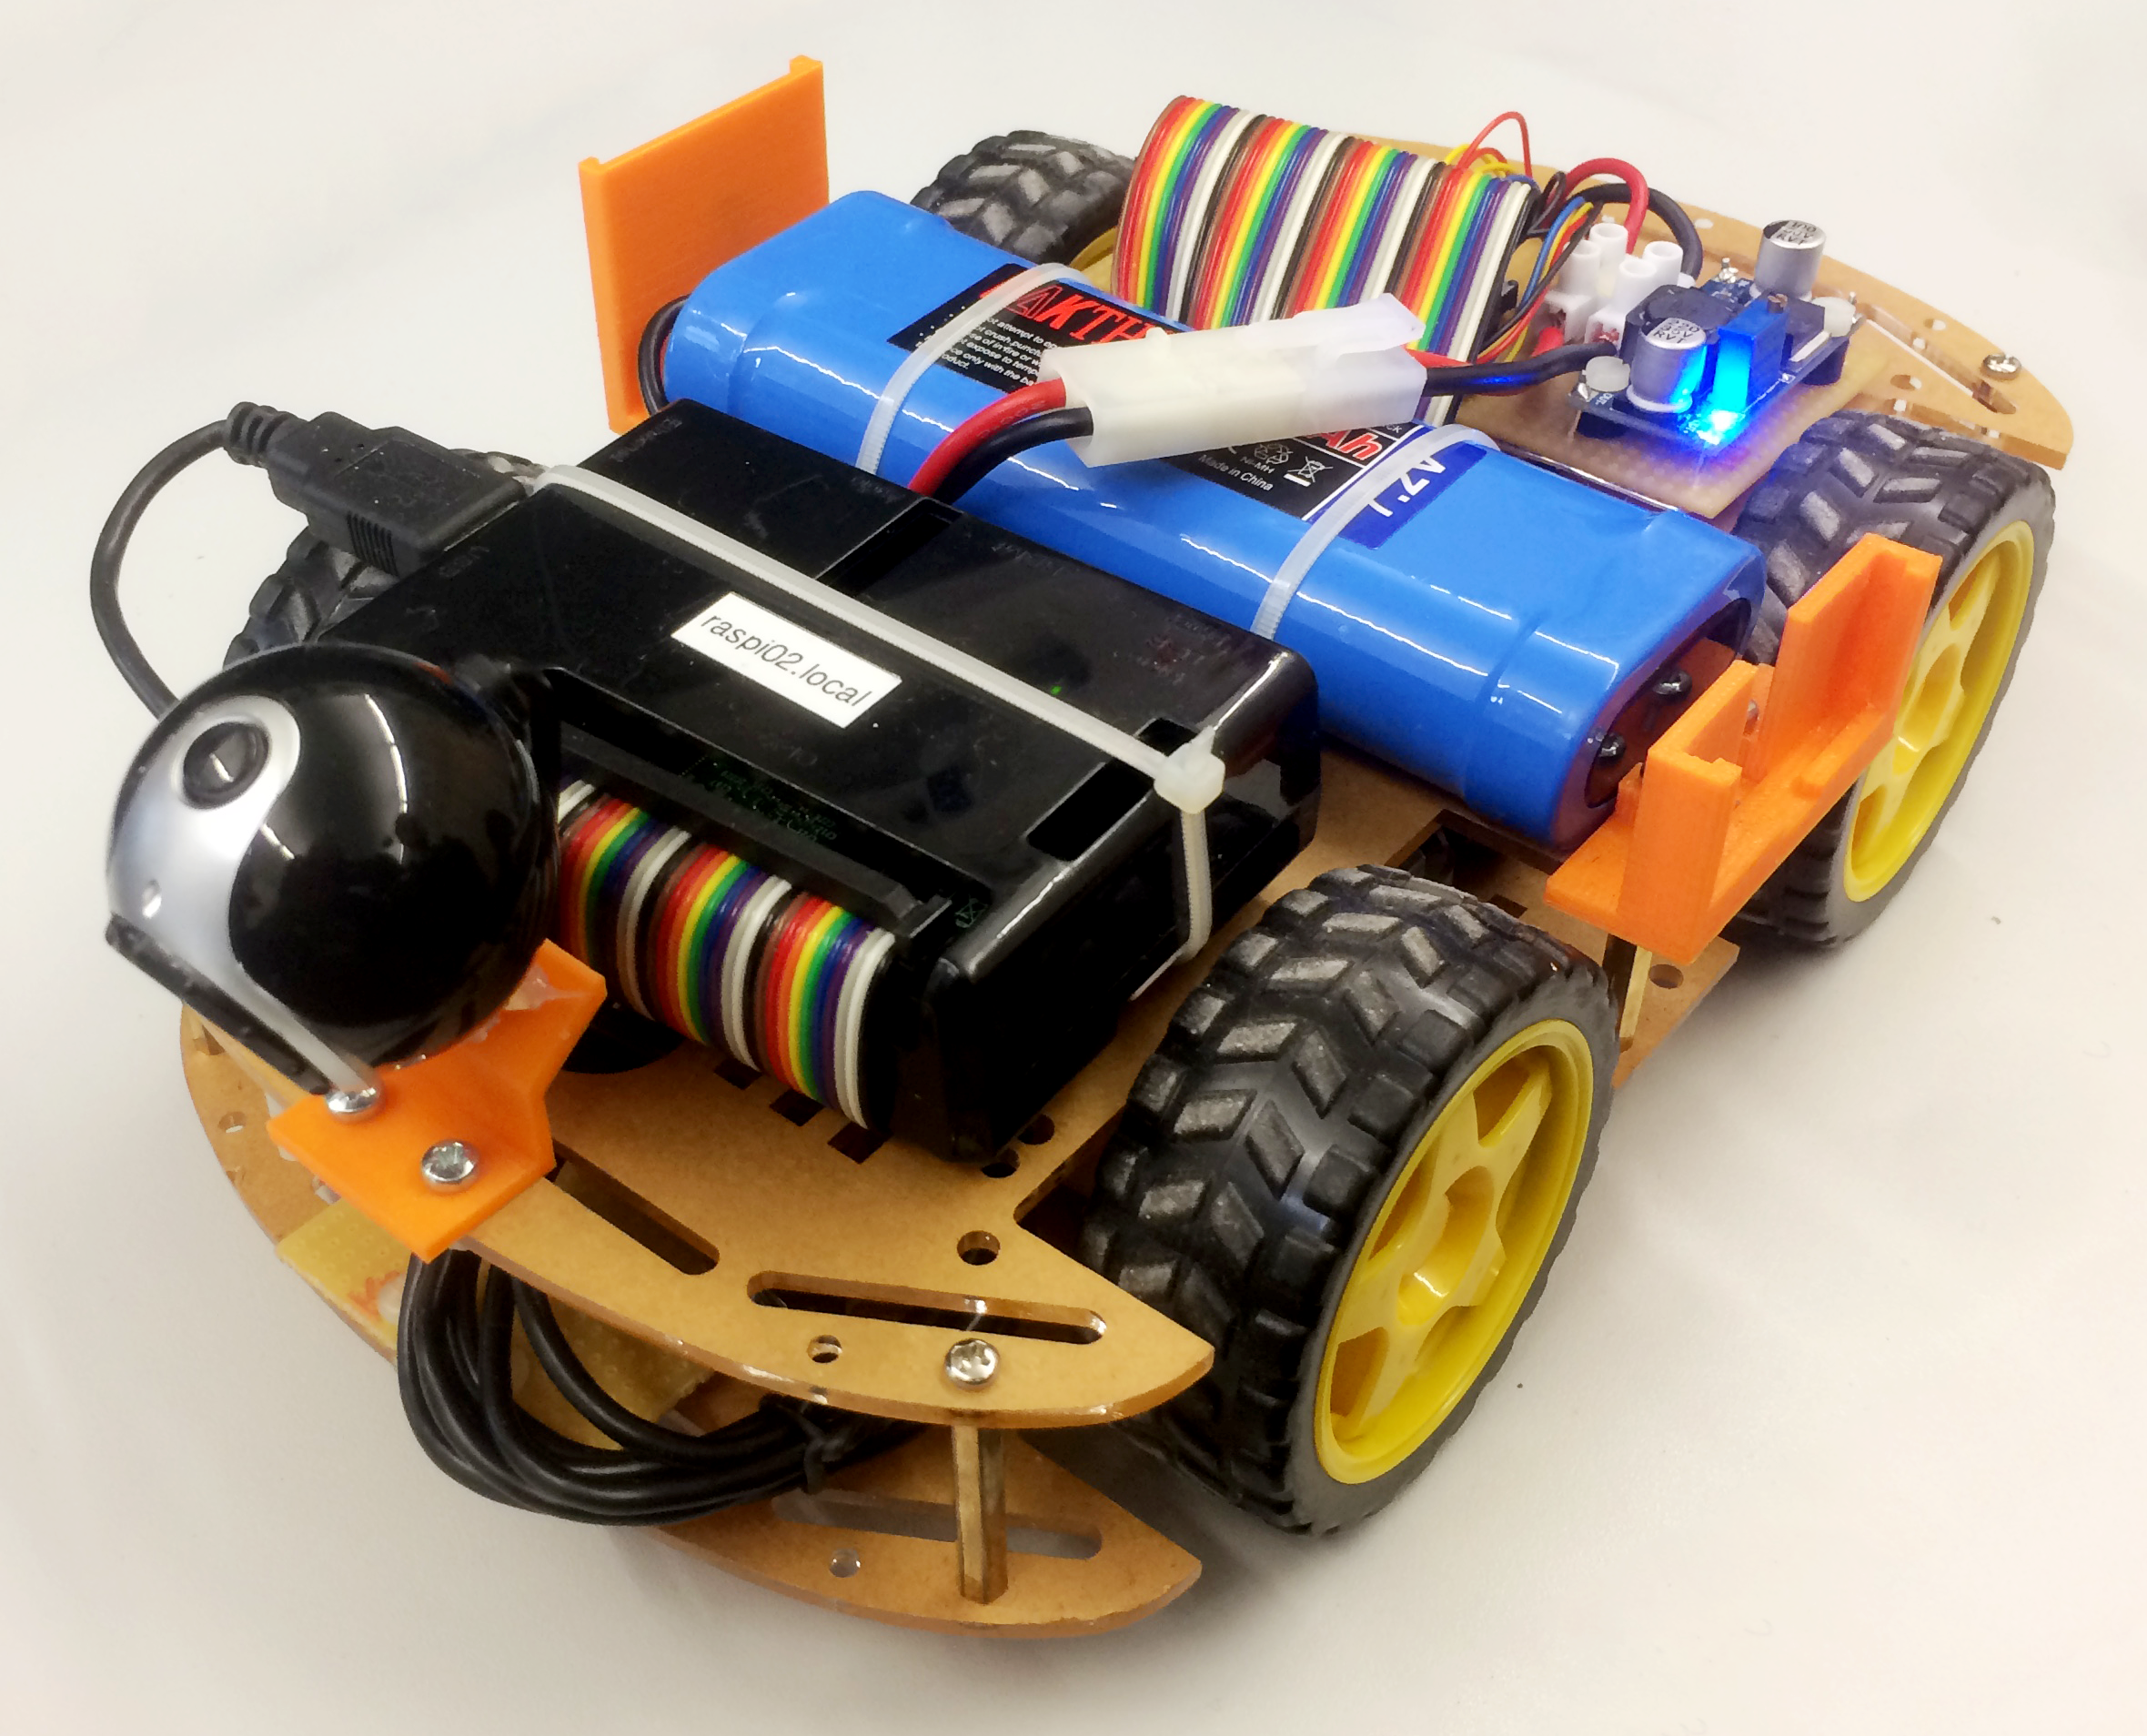
\includegraphics[width=\textwidth]{../bilder_videos/RaspberryCar.png}
	\end{subfigure}%
	\begin{subfigure}{.5\textwidth} 
		\centering
		\includegraphics[width=\textwidth]{../bilder_videos/RaspberryCar-2.png}
	\end{subfigure}%
	\caption{Das Auto im finalen Aufbau}
	\label{auto}
\end{figure}

Schon seit Beginn des Projekts sollten alle Bestandteile des Autos kompakt verbaut werden. Die Bauteile wurden fest angebracht und sind so angeordnet, dass sie das Gewicht des Autos gleichmäßig verteilen. Auf besondere äußerliche Ausstattungsmerkmale wurde deshalb bewusst verzichtet, um mehr Geschwindigkeit zuzulassen und die Motoren weniger zu belasten.

\subsection{Programmierung}

Da die Rennstrecke im Wesentlichen daraus besteht, einer roten Linie zu folgen, haben wir uns bereits früh mit der Bildverarbeitung beschäftigt. Dabei wurde in der Gruppe parallel an der Wandfahrt mit den Ultraschallsensoren und an der Linienfahrt mit der Kamera gearbeitet.

Das Auto soll sich in der Fahrweise der Strecke so anpassen, dass es bei geraden Abschnitten mit Höchstgeschwindigkeit fährt und je nach Kurvenradius etwas langsamer werden muss, ohne viel an Tempo zu verlieren. Die Lenkung ist ebenfalls, je nach Position der roten Linie, unterschiedlich stark und soll dennoch überall sanft und stufenlos geregelt werden. Hierfür setzt man die veränderliche Position der roten Linie ins Verhältnis zum theoretischen Idealwert des Mittelpunktes und berechnet daraus die Lenkung und Geschwindigkeit.

Nachdem das Grundgerüst für die Linienfahrt innerhalb weniger Wochen erarbeitet wurde, gab es genug Zeit für die Optimierung des Algorithmus. Funktionen wie die Erkennung von verschiedenfarbigen Ampeln oder die Videoaufnahme während der Fahrt wurden erst am Schluss hinzugefügt.

\subsection{Schaltplan}

\begin{figure}[H] 
	\centering
	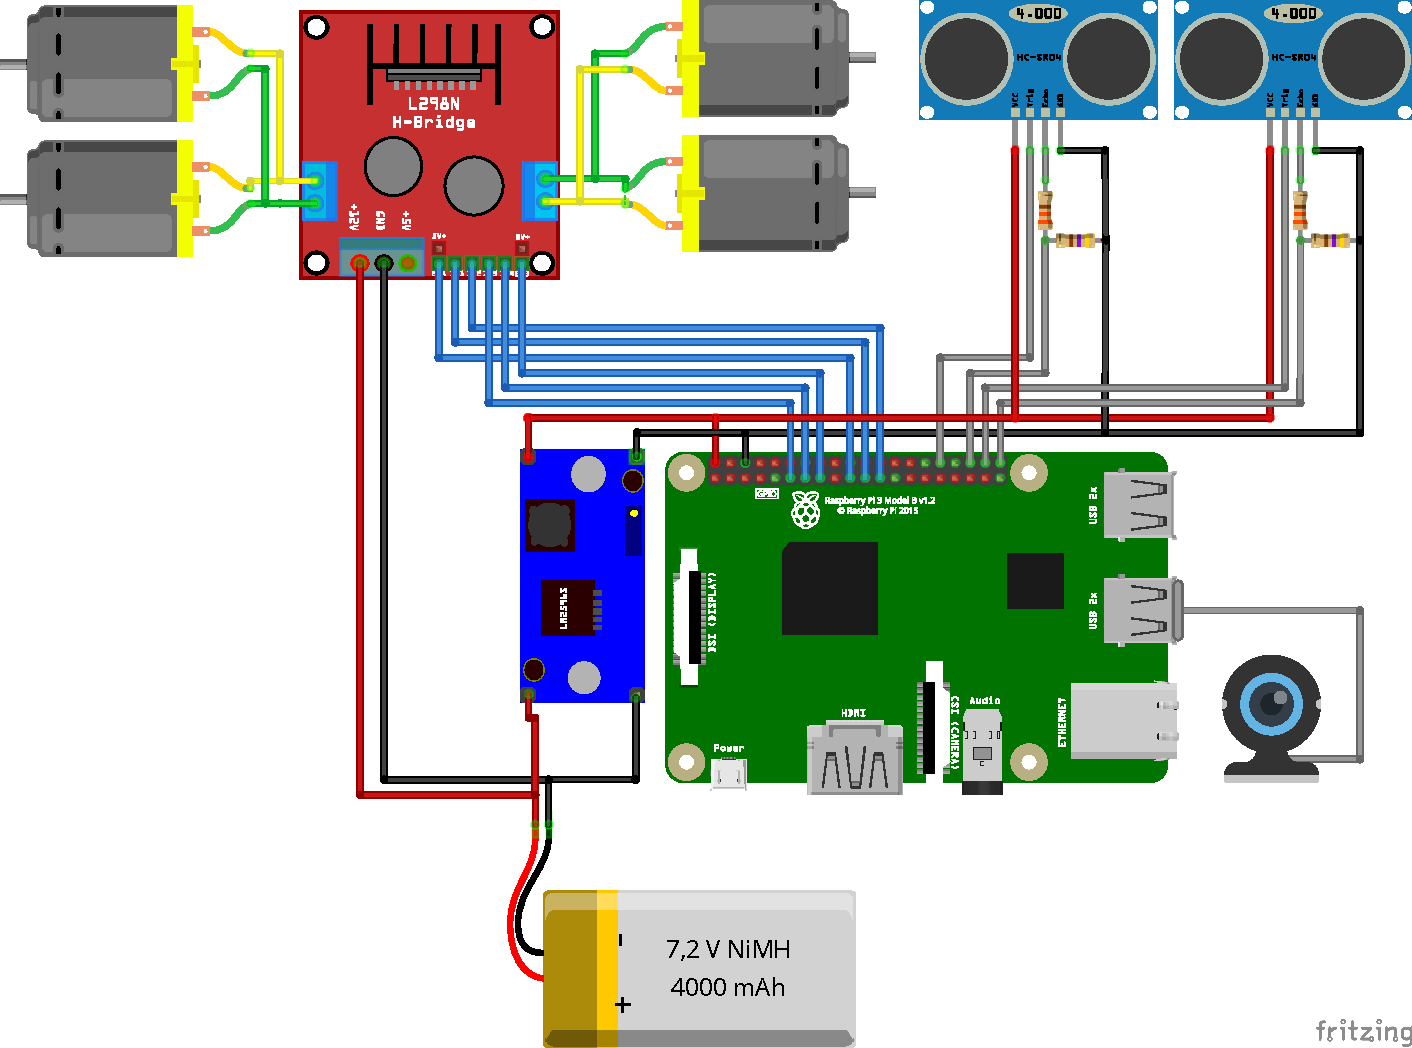
\includegraphics[width=.75\textwidth]{Schaltplan.pdf}
	\caption{Schaltplan}
	\label{schaltplan}
\end{figure}

In dem Auto sind insgesamt vier DC-Motoren verbaut, die in zwei Seiten links und rechts eingeteilt werden. Um die Motoren über den Raspberry Pi anzusteuern, werden sie jeweils als Gruppe an die Dual-H-Bridge angeschlossen, die als Motortreiber dient. Darüber kann mithilfe einer einfachen Logiktabelle die Stellung des Schalters und damit die Bewegung der Motoren eingestellt werden.

Die Ultraschallsensoren SC-HR04 arbeiten mit einem High-Pegel von \unit[5]{V}. Für den Echo-Pin, der mit dem Raspberry Pi verbunden ist, muss zwingend ein Spannungsteiler verwendet werden, da die GPIOs vom Raspberry Pi nur maximal eine Spannung von \unit[3,3]{V} erlauben. Die Webcam wird per USB angeschlossen.

Die gesamte Stromversorgung des Autos läuft über den \unit[4000]{mAh} großen Akku. Der eingebaute Gleichspannungsregler sorgt dafür, dass nur \unit[5]{V} am Raspberry Pi und den Sensoren anliegen.

\section{Code}

Das Programm wird über die Datei \textit{main.py} ausgeführt. Zwei Module \textit{setup.py} und \textit{aufrauemen.py} sind ausgelagert, dadurch ist die Hauptdatei übersichtlicher und die Module können einfacher von anderen Dateien mitbenutzt werden.

\subsection{main.py}

In \textit{main.py} wird das Modul \textit{Threading} verwendet, was gleich mehrere Vorteile hat. Die Bildaufnahme ist außerordentlich schneller, wenn sie auf einem anderen Thread als der restliche Algorithmus läuft und das Abspeichern der Bilder für eine Videoausgabe würde ohne das Threading die Rechendauer um ein Vielfaches erhöhen. Außerdem können so andere Funktionen unabhängig von dem restlichen Programm problemlos ausgeführt werden.

Es laufen drei Threads parallel: Der eigentliche Fahralgorithmus \textit{linienfahren}, die Videoausgabe \textit{makevideo} und die Ampelüberprüfung \textit{checkblue}. \textit{linienfahren} ruft zwei Funktionen auf, \textit{line} zur Bildaufnahme und \textit{lenken} zur Motorsteuerung.

Es werden mehrere globale Variablen zwischen den einzelnen Threads benutzt. Zum einen die Bildvariablen \textit{ret} und \textit{img}, damit nicht jede Funktion eigene Bilder aufnehmen muss und zum anderen der Linienmesswert \textit{x} und die verstrichene Zeit \textit{minutes, seconds}, die zur Videoausgabe benötigt wird.

\subsubsection{import}
\lstinputlisting[language=Python,firstline=1,lastline=14,caption={}]{../main.py}

Am Anfang der Hauptdatei werden die erforderlichen Module importiert, gefolgt von den beiden ausgelagerten Dateien. Von \textit{aufrauemen.py} werden die benötigten Funktionen und von \textit{setup.py} wird alles importiert, da diese Datei keine Funktion enthält. In den Zeilen 10 bis 14 werden die notwendigen Einstellungen für OpenCV vorgenommen und die Kameraausgabe vorbereitet.

\subsubsection{main}
\lstinputlisting[language=Python,firstline=167,caption={}]{../main.py}

Das Programm wird in \textit{main} gestartet und beendet. Als erstes werden die Motoren mit der Funktion \textit{losfahren} gestartet, allerdings noch mit einem Tastverhältnis von \unit[0]{\%}.
Anschließend wird das Threading aktiviert. Dafür wird \textit{run\_event}, das als \textit{while}-Bedingung für die Threads dient, gesetzt. Die Delay-Angaben und die drei verwendeten Threads \textit{th1}, \textit{th2} und \textit{th3} werden definiert. Dabei ist \textit{target} die Funktion, die in dem neuen Thread laufen soll und \textit{args} sind die Variablen, die mit übergeben werden.

Der erste Thread (die Videoaufzeichnung) wird gestartet, gefolgt von einer \textit{while}-Schleife, die überprüft, ob die Ampel grün ist. Wenn der zurückgegebene Wert der \textit{checkgreen}-Funktion größer gleich 500 ist, also ausreichend Grünanteile erkannt wurden, endet die Schleife. Dadurch werden die anderen beiden Threads gestartet, wodurch das Auto losfährt.

Damit das Programm wieder beendet werden kann, folgt eine \textit{try-while}- und \textit{except}-Schleife, die weiterhin keine andere Funktion hat. Sobald ein \textit{KeyboardInterrupt} durch das Drücken von Strg-C auftritt, bremst das Auto und die Threads werden geschlossen. Allerdings muss dabei gewartet werden, bis die \textit{while}-Schleifen aller Threads durchgelaufen sind. Anschließend werden die GPIO-Einstellungen bereinigt, die Videoaufnahme beendet und das Video gespeichert.

Gestartet wird die \textit{main}-Funktion durch die Abfrage \textit{if \_\_name\_\_ == "\_\_main\_\_"}, um die Datei auch als Modul verwenden zu können.

\subsubsection{line}
\lstinputlisting[language=Python,firstline=104,lastline=119,caption={}]{../main.py}

In \textit{line} wird für eine Bildzeile der Mittelpunkt der roten Anteile ermittelt. Hierfür wird zunächst ein Bild von der Webcam mit der \textit{cap.read()}-Funktion aufgenommen und als Variable definiert, wodurch das Bild nicht abgespeichert werden muss. 

Der Funktion wird beim Aufrufen nur die Zeile 70 (\textit{zeileNr}) übergeben, die sich für unsere Kameraposition besonders gut eignet, um bereits frühzeitig Kurven zu erkennen. Alle anderen Zeilen sind für die Bildverarbeitung nicht relevant und würden den Algorithmus verlangsamen. Außerdem wird ermöglicht, dieselbe Funktion zum Analysieren unterschiedlicher Zeilen zu verwenden. Dies wird in der finalen Version aber nicht benutzt, da das Auslesen einer einzigen Zeile zu keinem dauerhaften Verlust der Linie führt.

Als erstes werden die drei Farbkanäle B, G und R aus dem Bild extrahiert (Zeile 5--7). Es lässt sich nicht nur anhand des Rotkanals feststellen, ob die Linie im aufgenommenen Bild wirklich rot ist, da zum Beispiel die Farben Weiß und Gelb ebenfalls einen Rotanteil von \unit[100]{\%} besitzen. Dennoch kann die „Rotheit“ des Bildes durch folgende Formel einfach berechnet werden:
\begin{equation}
\text{Rotheit} = R-\frac{G+B}{2}
\end{equation}

Durch die Anwendung der Formel wird nur eine hohe Rotheit erzielt, wenn im Bild auch ein rotes Pixel vorliegt. Die Umrechnung zum Datentyp \textit{int16} ist erforderlich, damit bei Überschreitung des Wertes 255 noch Platz nach oben ist (bis 16 Bit) und nicht fälschlicherweise wieder bei null weitergezählt wird.

Die Festlegung eines Schwellwertes, in diesem Fall 60, hat den Zweck, die niedrigen Rotwerte herauszufiltern, die nicht Teil der Linie sind. Die Variable \textit{zeile\_bin} gibt dann als Ergebnis ein Array aus, in dem entweder \textit{True}- oder \textit{False}-Werte für die jeweiligen Pixel eingetragen sind  (Zeile 9). Danach wird durch Multiplikation der Variablen $x$ bestimmt, an welchen Positionen der Zeile jeweils ein \textit{True} ausgegeben wurde, also in welchem Bereich des Bildes die Linie zu finden ist. 

Für die Berechnung des Mittelpunktes wird genauer betrachtet die Formel des Schwerpunktes angewendet. Dafür wird die Summe der $x$-Positionen aller Pixel mit einer Rotheit von über 60 durch die Anzahl dieser vorkommenden Pixel geteilt (Zeile 14). Dies entspricht genau der Mitte zwischen dem ganz linken und rechten Pixel der roten Linie.

Falls das Auto an einer Stelle die Linie verliert, werden auch keine roten Pixel gezählt. Für solche Fälle wurde zusätzlich die \textit{if}-Abfrage eingebaut, um eine Division durch Null auszuschließen. Als Ergebnis wird \textit{None} ausgegeben und im Hauptprogramm auf den letzten gültigen berechneten Mittelpunkt zurückgeführt.
\begin{figure}[H] 
	\centering
	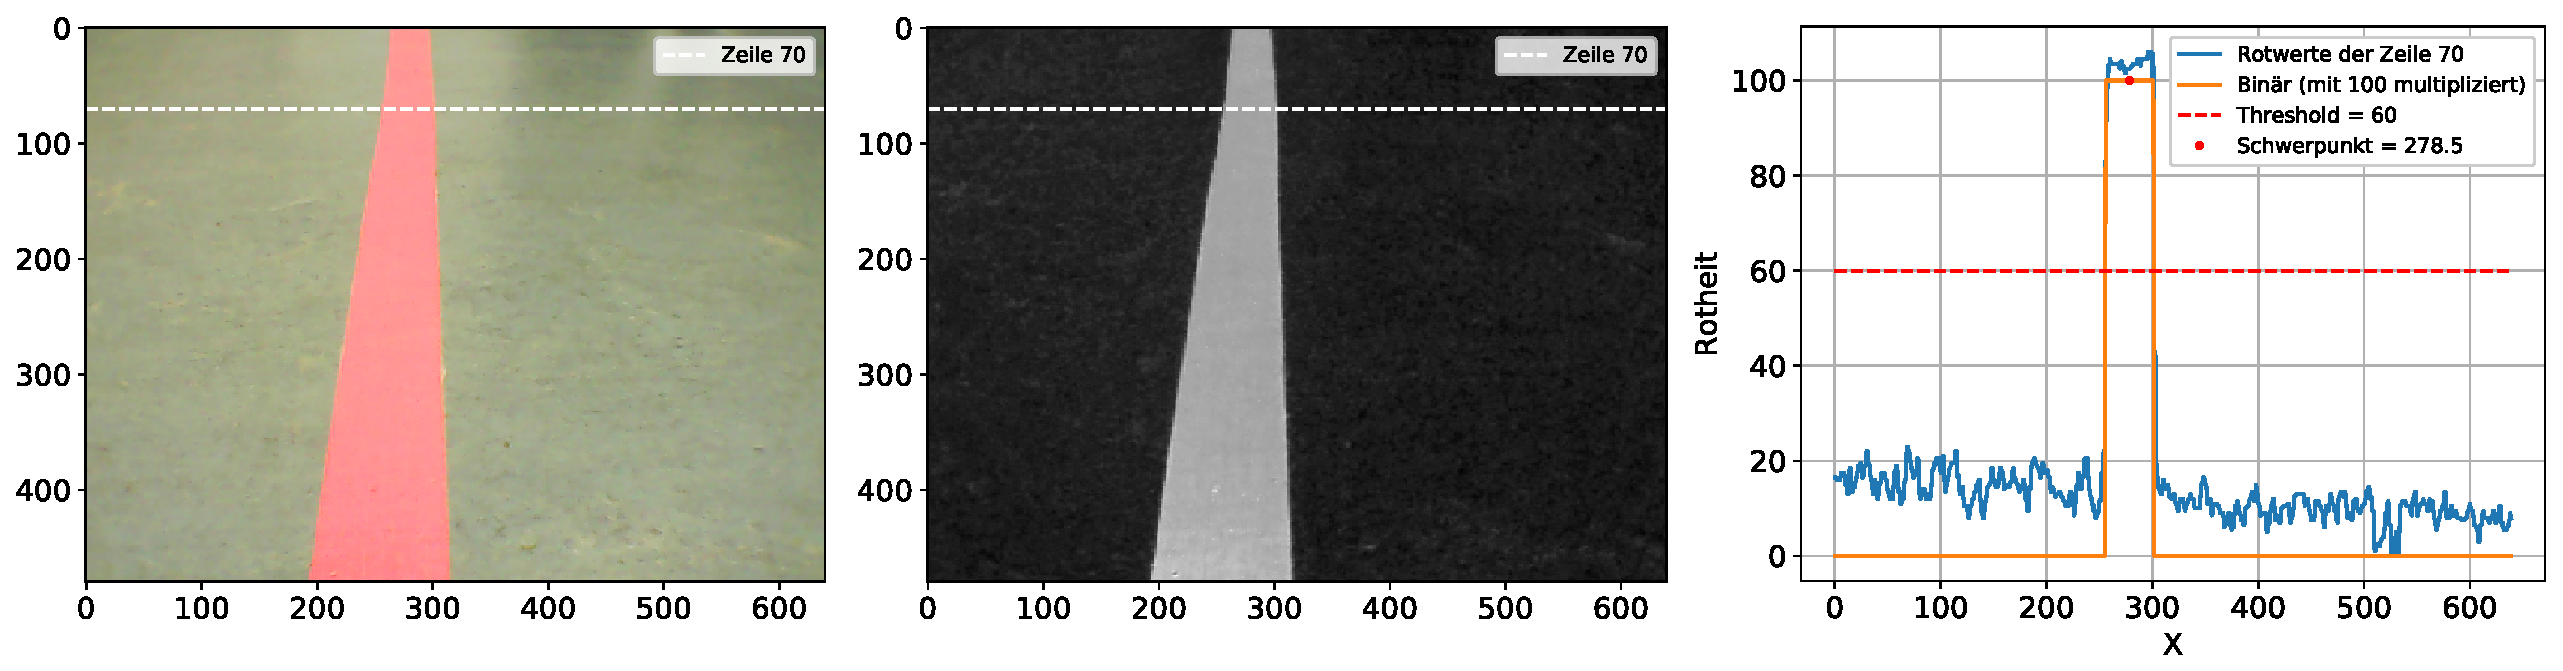
\includegraphics[width=1\textwidth]{Testbild.eps}
	\caption{Berechnung des Mittelpunktes für die Zeile 70}
	\label{mittelpunkt}
\end{figure}

Für das Testbild in Abbildung \ref{mittelpunkt} wird folgender Mittelpunkt in der Zeile 70 berechnet:

\begin{equation}
\text{Mittelpunkt} = \frac{ (\textit{zeile\_bin $*$ x}).\textit{sum}() }{ (\textit{zeile\_bin} ).\textit{sum}() } = \frac{12811}{46} = 278,5
\end{equation}

\newpage

\subsubsection{linienfahren}
\lstinputlisting[language=Python,firstline=122,lastline=164,caption={}]{../main.py}

\textit{linienfahren} ruft die Funktion \textit{line} auf und berechnet die Lenkung und Geschwindigkeit aus dem zurückgegebenen Wert.

Am Anfang der Funktion wird ein Testbild aufgenommen und die für die Berechnung benötigten Variablen erstellt. Danach folgt eine \textit{while}-Schleife, die bis zum Beenden des Threadings durchläuft.
Falls keine rote Linie im Bild war, oder in seltenen Fällen, wenn die Linie nicht erkannt wurde, gibt \textit{line} \textit{None} zurück. In diesem Fall wird in den Zeilen 17 bis 21 überprüft, ob die Linie zuletzt rechts oder links im Bild war. Der Messwert \textit{mitte} wird dementsprechend auf das Minimum (0) oder das Maximum (640) gesetzt, um bei Verlust der Linie schnell zu reagieren. Anschließend wird der Wert für die Videoausgabe abgespeichert (Zeile 22).

In den Zeilen 24 bis 33 wird der Wert für die Lenkung und Geschwindigkeit berechnet. Unterschieden wird zwischen drei Fällen: Ist der Messwert in der Mitte des Bildes, wird geradeaus gelenkt, andernfalls wird die Lenkung und die Geschwindigkeit berechnet. Ist der Messwert größer als der Bildmittelpunkt, wird $2-\textit{Lenkwert}$ gerechnet. Es ergibt sich ein Lenkwert zwischen 0 und 1 für eine Linkskurve und 1 bis 2 für eine Rechtskurve. Das hat den Vorteil, dass der \textit{lenken}-Funktion nicht zusätzlich eine Richtungsangabe übergeben werden muss. Anschließend wird die \textit{lenken}-Funktion mit den Lenk- und Geschwindigkeitsvariablen aufgerufen.

Der Wert für die Lenkung und die Geschwindigkeit wird aus dem Messwert und dem Bildmittelpunkt berechnet:
\begin{align}
\text{Lenkung}&=\frac{\text{Messwert}}{\text{Bildmittelpunkt}}\cdot\unit[90]{\%}+\unit[10]{\%}\\[2ex]
\text{Geschwindigkeit}&=\frac{\text{Messwert}}{\text{Bildmittelpunkt}}\cdot\unit[60]{\%} + \unit[40]{\%}
\end{align}
Damit die Lenkung nicht zu stark ist, wird der Wert kleiner gewichtet ($\cdot\unit[90]{\%}$) und angehoben ($+\unit[10]{\%}$). So startet der Wert nicht bei \unit[0]{\%}, sondern bei \unit[10]{\%}.
Die Geschwindigkeit wird gleich berechnet, allerdings mit ($\cdot\unit[60]{\%}$) gewichtet und ($+\unit[40]{\%}$) angehoben. Es wird also immer mit \unit[40]{\%} bis \unit[100]{\%} Geschwindigkeit gefahren.

Für die Text- und Videoausgabe wird die verstrichene Zeit berechnet. Anschließend folgt in Zeile 40/41 eine Textausgabe über die Konsole. Dabei werden $\frac{\text{Messwert}}{10}$ Leerzeichen, dann ein Blockzeichen als Position des Messpunktes im Bild und die verbleibenden $64-\frac{\text{Messwert}}{10}$ Leerzeichen geschrieben. Dann folgen noch Angaben zu Messpunkt, Lenkwert, Geschwindigkeit und Zeit. In der nächsten Zeile wird der Mittelpunkt mit einem Strich markiert. Es ergibt sich eine Textausgabe, die zum Beispiel so aussieht:

\begin{lstlisting}[numbers=none]
               █                     x = 245.0 ;steer = 0.8 ;speed = 85.9 ;time = 00:00.00
                       |
                 █                   x = 265.0 ;steer = 0.8 ;speed = 89.7 ;time = 00:00.04
                       |
                   █                 x = 284.0 ;steer = 0.9 ;speed = 93.2 ;time = 00:00.08
                       |
                    █                x = 292.0 ;steer = 0.9 ;speed = 94.8 ;time = 00:00.12
                       |
                     █               x = 304.0 ;steer = 1.0 ;speed = 97.0 ;time = 00:00.16
                       |
                      █              x = 312.0 ;steer = 1.0 ;speed = 98.5 ;time = 00:00.20
                       |
                       █             x = 325.0 ;steer = 1.0 ;speed = 99.1 ;time = 00:00.24
                       |
\end{lstlisting}
\vspace{-4ex}
\subsubsection{lenken}
\lstinputlisting[language=Python,firstline=76,lastline=101,caption={}]{../main.py}

Die \textit{lenken}-Funktion steuert das Tastverhältnis der Motoren. Übergeben werden zwei Parameter für die Lenkgewichtung und die Geschwindigkeit. Am Anfang der Funktion werden einige Abfragen zur Fehlerverhütung vorgenommen, damit das Tastverhältnis nicht unter \unit[0]{\%} oder über \unit[100]{\%} liegt, dies würde sonst zu einem Absturz führen.

Damit das Auto in den Kurven nicht ungewollt langsamer fährt, wird ausgerechnet, wie viel schneller sich die äußeren Motoren drehen können.
\begin{align}
\text{Kopfraum} = 100-\text{Geschwindigkeit}
\end{align}
Ist der Kopfraum größer als der Geschwindigkeitswert, wird der Kopfraum gleich der Geschwindigkeit gesetzt.

Die Tastverhältnisse der Motoren werden gleich dem Geschwindigkeitswert gesetzt, wenn der Lenkwert $steer=1$ ist. Sonst wird unterschieden, ob der Lenkwert größer oder kleiner als 1 ist, um in die entsprechende Richtung zu lenken.
\begin{align}
	&\text{Innere Motoren:} &\text{Tastverhältnis} &= \text{Lenkwert}\cdot\text{Geschwindigkeit}\\
	&\text{Äußere Motoren:} &\text{Tastverhältnis} &= (1-\text{Lenkwert})\cdot\text{Kopfraum}+\text{Geschwindigkeit}
\end{align}
Die Kombination aus dem Lenkwert, Geschwindigkeitswert und Kopfraum ermöglicht ein stufenloses Kurvenfahren, ohne dass an Geschwindigkeit verloren wird. Dabei ist es egal, worauf die Werte basieren, es wird immer gleich sanft gelenkt.

\begin{table}[H]
	\centering
	\begin{tabular}{c|c|c|c}
		Lenken & Geschwindigkeit & $T_{\text{innen}} [\%]$ &  $T_{\text{außen}}[\%]$ \\ \hline 
		0,2 & 20 & \ 2 & 36 \\  
		    & 60 & 12  & 92 \\    
		    & 80 & 16  & 96 \\ \hline
		0,8 & 20 & 16  & 24 \\
		    & 60 & 48  & 68 \\
		    & 80 & 64  & 84 \\
	\end{tabular} 
	\caption{Beispielwerte für die Motorensteuerung}
\end{table}

\subsubsection{checkgreen}
\lstinputlisting[language=Python,firstline=36,lastline=50,caption={}]{../main.py}

Die \textit{checkgreen}-Funktion ist eine einfache Methode zur Erkennung einer grünen Ampel. Sie analysiert ein ganzes Bild der Webcam auf ihren Grünanteil und gibt die Anzahl der Pixel in einem gewählten HSV-Bereich an. Dabei ist zu beachten, dass die Funktion nur auf die Farbe der Ampel reagiert und nicht einen Fehlstart des Autos durch andere Grüntöne im Bild auslöst. Um dies zu vermeiden, wird eine Umwandlung des Farbraums von BGR -- was die Kamera nativ ausgibt -- zu HSV vorgenommen (Zeile 8), um einen präzisen Farbbereich mit zwei Threshold-Werten für die untere und obere Grenze mithilfe von OpenCV festzulegen. Danach wird eine Maske mit der Funktion \textit{cv2.inRange} erstellt, in der alle Pixel innerhalb dieses Farbbereichs liegen (Zeile 13).
Um festzustellen, dass die Ampel im Bild grün ist, werden alle weißen Pixel der Maske mit \textit{cv2.countNonZero} gezählt (Zeile 14). Erst bei einer genügend großen Anzahl an grünen Pixeln, hier mehr als 500, beginnt das Auto die Fahrt.

Der HSV-Raum eignet sich im Gegensatz zu BGR gut für die Selektion eines Farbbereiches, weil er sich aus drei Komponenten Hue (Farbton), Saturation (Farbsättigung) und Value (Hellwert) zusammensetzt. Als Testbild wurde mit der Webcam ein Bild des LED-Streifens aufgenommen, wobei zusätzlich noch ein ähnlicher Farbton in Form eines grünen Klebebandes dazukommt, um die Grenzen besser festzulegen. Für die Umrechnung von BGR- nach HSV-Werten gelten je nach Formelsatz andere Intervalle. Die Tabelle \ref{hsv} zeigt einen Vergleich zwischen gängigen Bildbearbeitungsprogrammen und OpenCV:

\begin{table}[H]
	\centering
	\begin{tabular}{l|l|l}
		Komponente & Bildbearbeitungsprogramm & OpenCV
		\\
		\hline
		Hue (Farbton) & $H\in\left[0^\circ, 360^\circ\right]$ & $H\in\left[0, 179\right]$
		\\
		Saturation (Farbsättigung) & $S\in\left[0, 1\right]$ & $S\in\left[0, 255\right]$
		\\
		Value (Hellwert) & $V\in\left[0, 1\right]$ & $V\in\left[0, 255\right]$
	\end{tabular} 
	\caption{Intervalle des HSV-Farbraums}
	\label{hsv}
\end{table}

Eine schnelle Umrechnung von BGR (Werte zwischen 0 und 255) nach HSV lässt sich durch folgende Befehle umsetzen:

\begin{lstlisting}
import cv2
import numpy as np
bgr_color = np.uint8([[[B,G,R]]])
hsv_color = cv2.cvtColor(bgr_color,cv2.COLOR_BGR2HSV)
print(hsv_color)
\end{lstlisting}

\begin{figure}[H]
	\centering
	\begin{subfigure}{.5\textwidth}
		\centering
		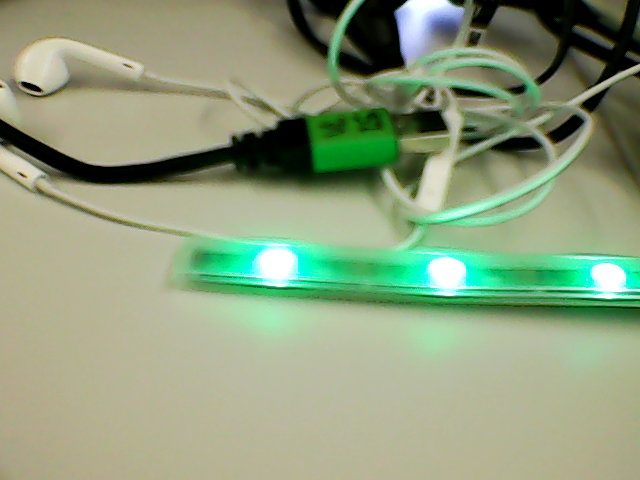
\includegraphics[width=\textwidth]{../testbilder/gruen.png}
	\end{subfigure}%
	\begin{subfigure}{.5\textwidth}
		\centering
		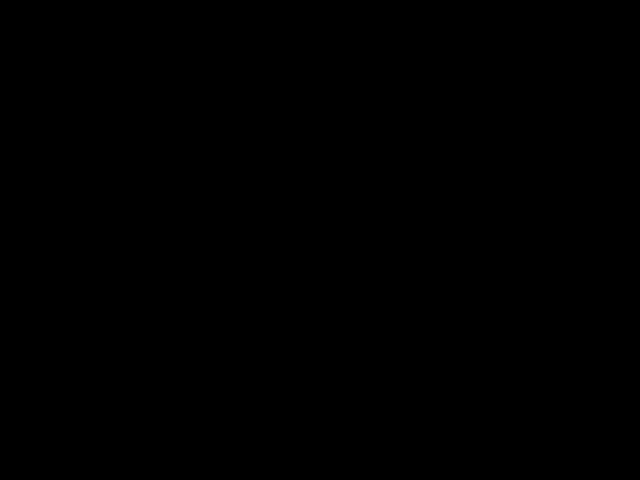
\includegraphics[width=\textwidth]{../testbilder/gruen2.png}
	\end{subfigure}
	\vspace{1ex}
	
	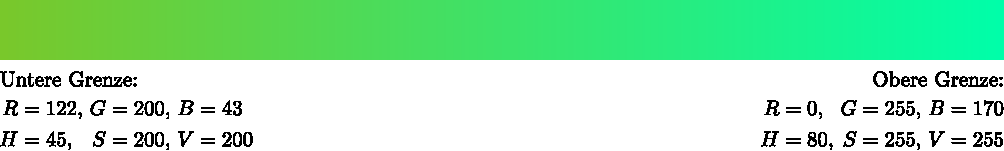
\includegraphics[width=1\textwidth]{../testbilder/Gruen_Bereich.pdf}
	\caption{Erkennung der grünen Ampel}
\end{figure}

Nach der Funktion werden 2616 grüne Pixel für den gewählten Bereich gezählt, die nur das Licht von den LEDs einschließen und nicht das grüne Klebeband. Es war auch darauf zu achten, dass unser Auto nur bei einer grünen und nicht auch bei einer blauen Ampel losfährt, da die LEDs auf dem Kamerabild teilweise ins Türkis und Hellgrün hineinragen.

\subsubsection{checkblue}
\lstinputlisting[language=Python,firstline=53,lastline=73,caption={}]{../main.py}

\textit{checkblue} funktioniert ähnlich wie \textit{checkgreen}, allerdings läuft die Funktion in Dauerschleife und stoppt das Auto nach 1,5 Sekunden, nachdem die blaue Ampel erkannt wurde. Dies hat den einfachen Grund, dass das Auto nicht sofort bei Erkennung der blauen Ampel vor der Ziellinie stehen bleibt, sondern diese sicher überschreiten kann. Die Funktion nimmt dabei kein eigenes Bild auf, sondern verwendet das Bild, das von der \textit{linienfahren}-Funktion aufgenommen wurde. Beim Starten des Threads wartet die Funktion eine Sekunde, damit die grüne Ampel nicht fälschlicherweise als Stoppsignal erkannt wird.

\begin{figure}[H]
	\centering
	\begin{subfigure}{.5\textwidth}
		\centering
		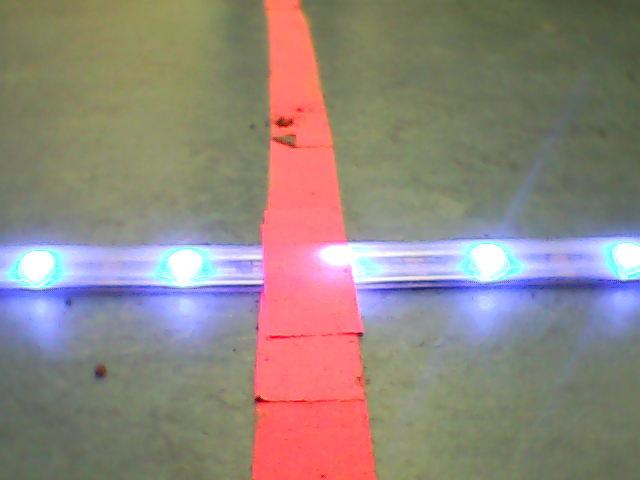
\includegraphics[width=\textwidth]{../testbilder/blau.png}
	\end{subfigure}%
	\begin{subfigure}{.5\textwidth}
		\centering
		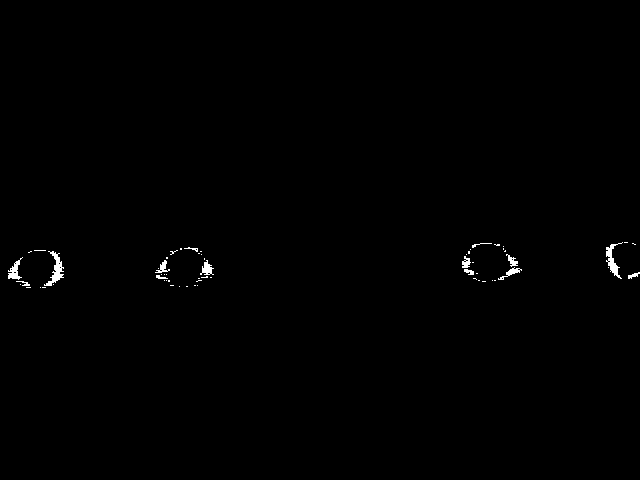
\includegraphics[width=\textwidth]{../testbilder/blau2.png}
	\end{subfigure}
	\vspace{1ex}

	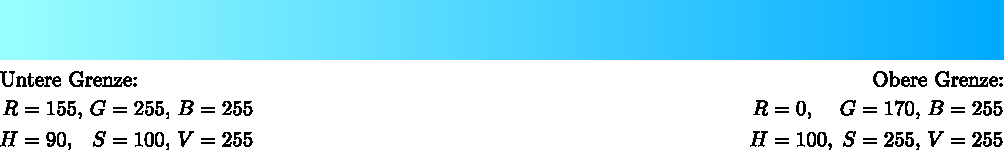
\includegraphics[width=1\textwidth]{../testbilder/Blau_Bereich.pdf}
	\caption{Erkennung der blauen Ampel}
\end{figure}


\subsubsection{makevideo}
\lstinputlisting[language=Python,firstline=17,lastline=33,caption={}]{../main.py}

Die Aufgabe der \textit{makevideo}-Funktion ist es, die von der Kamera aufgenommenen Bilder als ein Video zu exportieren. Da das Video nur zur Fehleranalyse und Veranschaulichung dient, wird es vernachlässigt, ob das Video in Echtzeit läuft. Dafür wird die aktuelle Fahrzeit -- ab dem Erkennen der grünen Ampel -- unten links im Bild eingeblendet. Außerdem wird der zu dem Bild gehörende Messpunkt und dessen Wert eingezeichnet.

Das Video in Zusammenhang mit den eingeblendeten Werten ermöglicht eine deutlich bessere Fehleranalyse als eine Textausgabe über die Konsole (Abb. \ref{schuh_im_bild}).

\begin{figure}[H] 
	\centering
	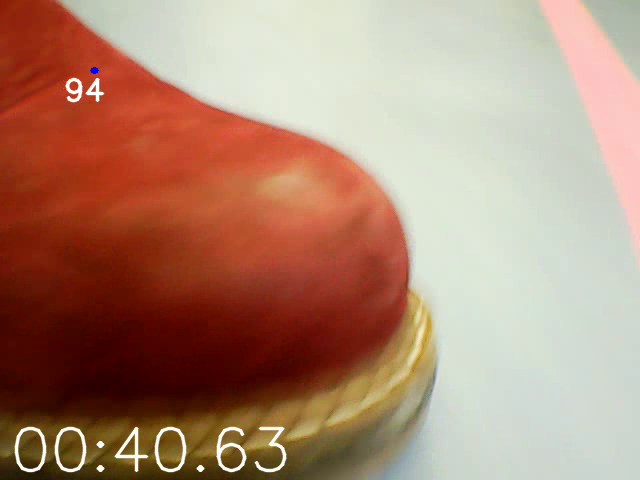
\includegraphics[width=.5\textwidth]{schuh_im_bild.png}
	\caption{Kamerabild mit Zeitanzeige und Messpunkt, abgelenkt von einem roten Schuh}
	\label{schuh_im_bild}
\end{figure}

\subsection{setup.py}
\lstinputlisting[language=Python,caption={}]{../setup.py}

In \textit{setup.py} werden die GPIOs definiert, das Skript wird am Anfang von \textit{main.py} aufgerufen. Verwendet wird der BCM-Modus. Für die PWM wurde eine Frequenz von \unit[73]{Hz} gewählt, was mit den Ultraschallsensoren zusammenhängt.

Dadurch, dass das GPIO-Setup ausgelagert war, konnten alle Python-Skripte während der ganzen Entwicklungsphase problemlos verwendet werden. Wenn die GPIOs sich ändern, muss dies nur in dieser einen Datei eingetragen werden.

\subsection{aufraeumen.py}
\lstinputlisting[language=Python,caption={}]{../aufraeumen.py}

In \textit{aufrauemen.py} sind drei Funktionen ausgelagert. \textit{losfahren} setzt die vier GPIOs der Motoren auf die entsprechenden Werte zum Vorwärtsfahren, \textit{bremsen} setzt die GPIOs zum Stoppen des Autos auf null und \textit{aufrauemen} stoppt das Auto und bereinigt die GPIO-Einstellungen.

\section{3D-Druck-Halterungen}

\subsection{Kamerahalterung}

Um die Kamera besser in das Auto integrieren zu können und um ein ständiges Nachjustieren zu umgehen -- da die Kamera bei Anbringung vor dem Auto immer verstellt wird, wenn ein Unfall gebaut wird -- wurde eine spezielle Halterung entwickelt. Diese erlaubt die Positionierung der Kamera oberhalb unseres Autos und bietet somit mehr Sicherheit vor Hindernissen.

Erstellt wurde die Halterung mit dem Online-3D-Design-Tool Tinkercad. Da die Kamera auch mit dieser Halterung immer noch von Hindernissen erreicht werden konnte (zum Beispiel hervorstehenden Schrankwänden), wurde die Verbindung von Kamera und Halterung zusätzlich mit Sekundenkleber verstärkt. 

\begin{figure}[H] 
	\centering
	\begin{subfigure}{.25\textwidth} 
		\centering
		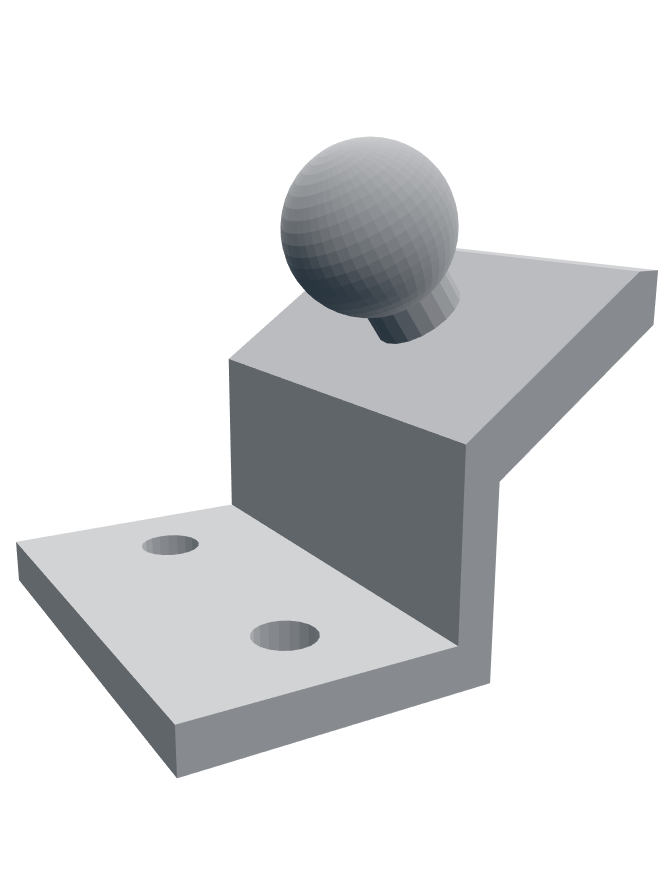
\includegraphics[width=\textwidth]{../3D-Druck_Modelle/Kamerahalterung_neu.png}
	\end{subfigure}%
	\begin{subfigure}{.25\textwidth} 
		\centering
		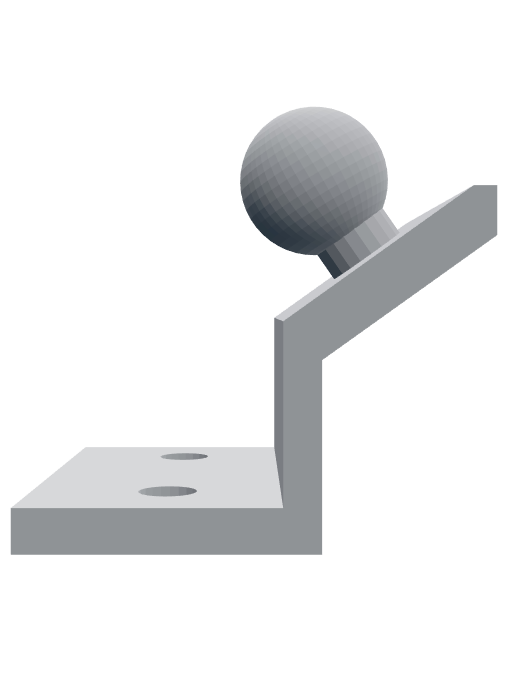
\includegraphics[width=\textwidth]{../3D-Druck_Modelle/Kamerahalterung_neu_top.png}
	\end{subfigure}%
	\hspace{2ex}
	\begin{subfigure}{.25\textwidth}
		\centering
		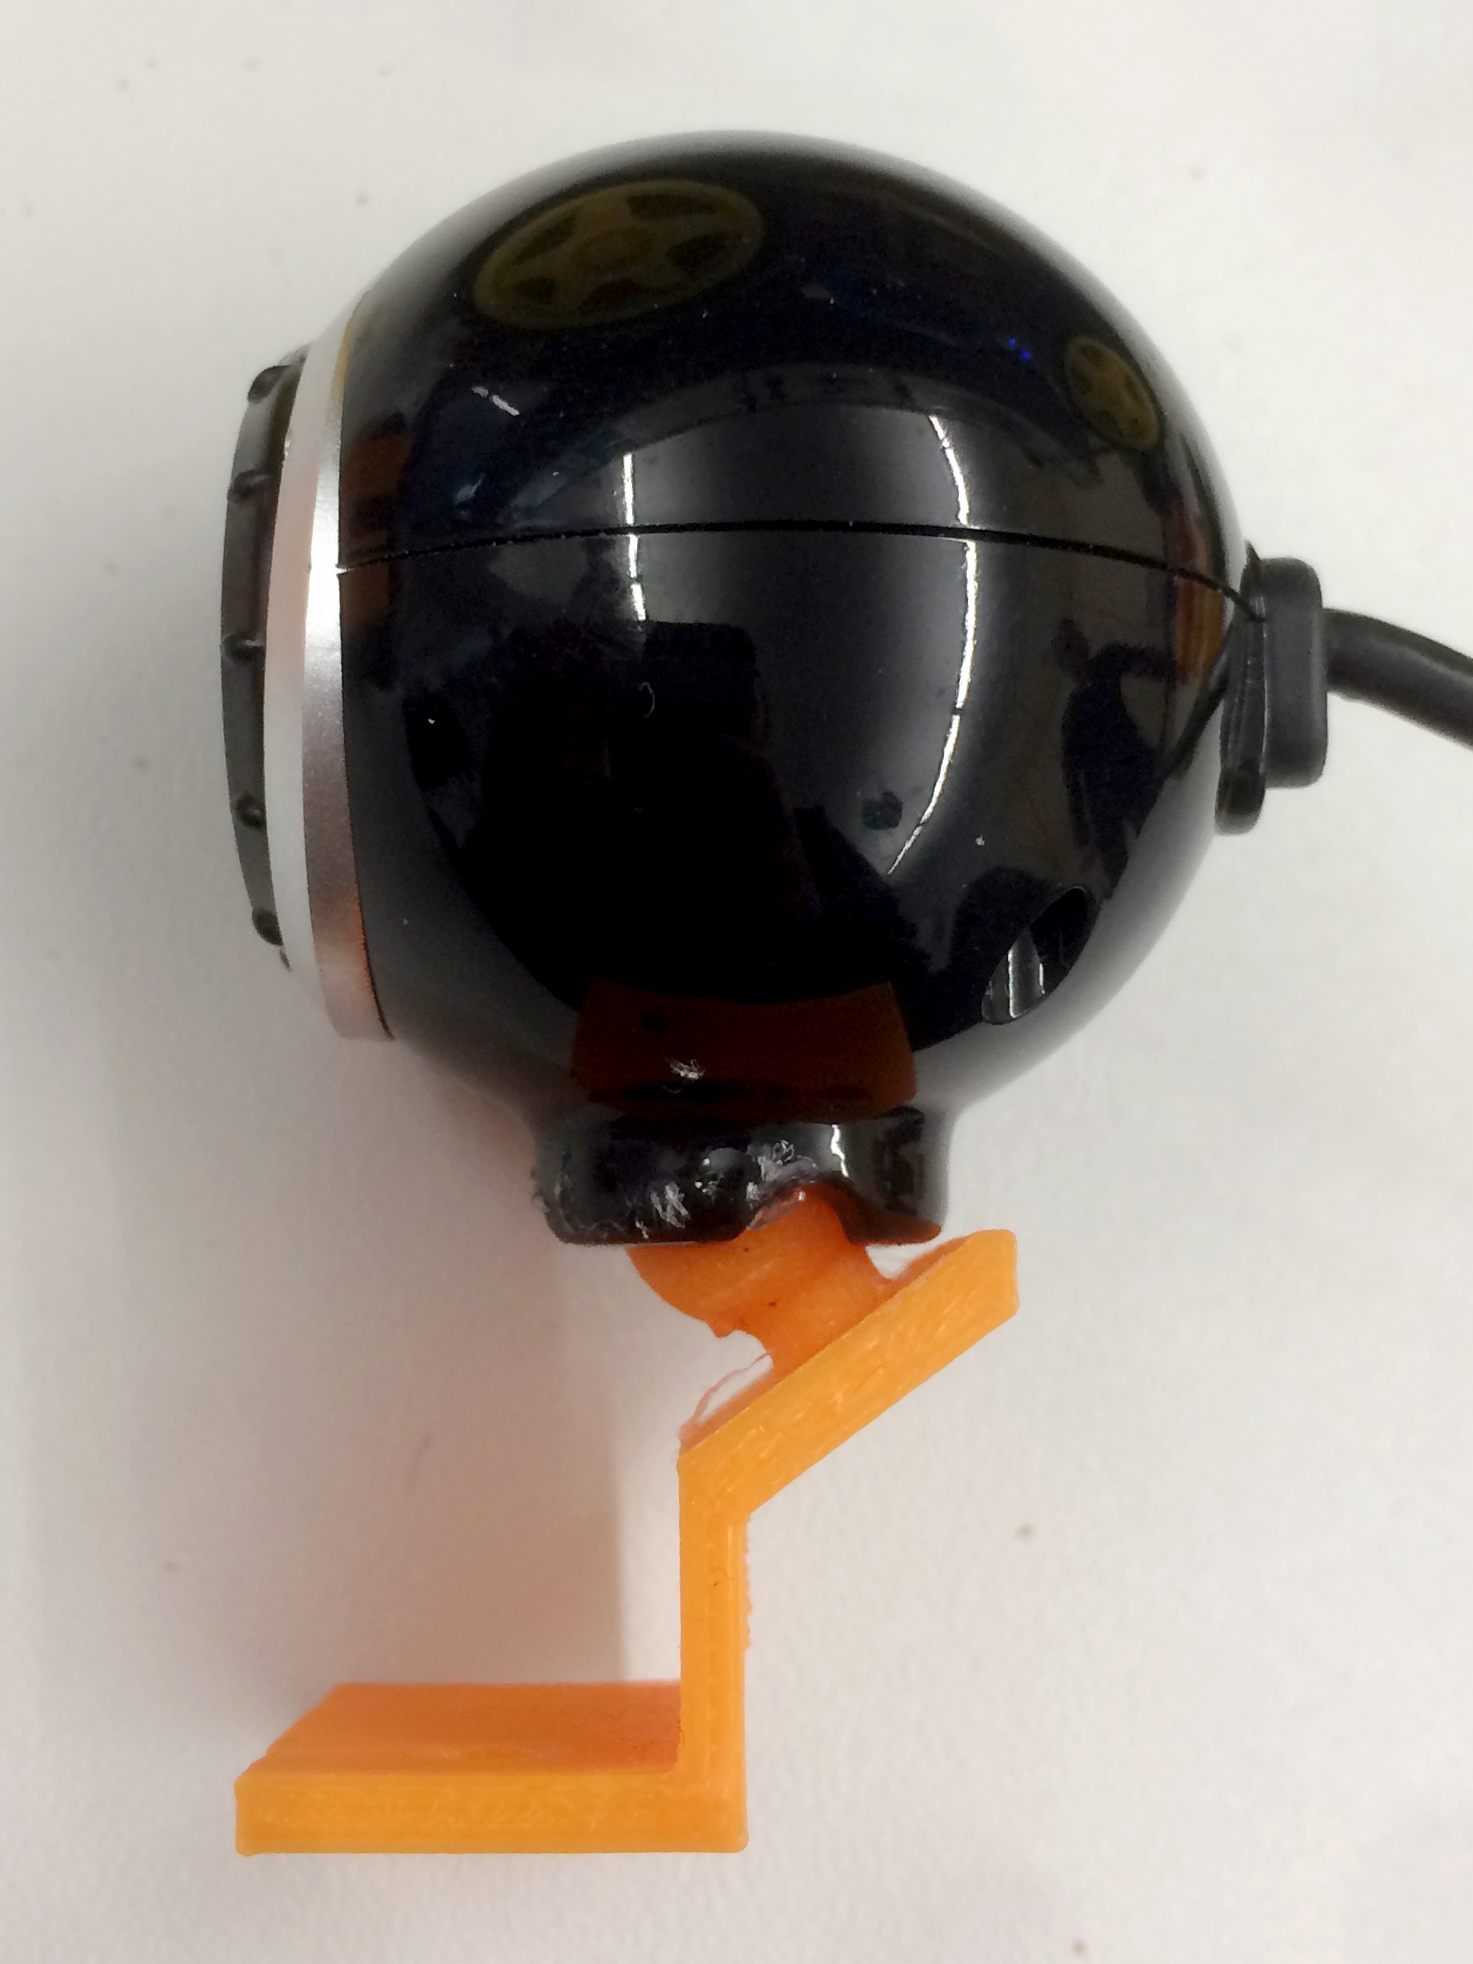
\includegraphics[width=\textwidth]{../bilder_videos/Kamerahalterung.png}
	\end{subfigure}%
	\caption{Kamerahalterung 3D-Modell und fertiger 3D-Druck}
	\label{kamerahalterung}
\end{figure}


\subsection{Ultraschallsensorhalterung}

Für den Ultraschallsensor HC-SR04 wurde eine Halterung entworfen, die es ermöglicht, den Sensor sowohl aufrecht als auch kopfüber an dem Auto zu befestigen. Außerdem sollte der Sensor, wie alle Teile des Autos, einfach abnehmbar sein, falls Änderungen vorgenommen werden müssen. Entworfen wurde das Modell in Blender 2.79 mit zwei Löchern für Schrauben, Platz für weitere Bohrungen und einen Schlitz für die Steckverbindung.

Der 3D-Druck ging problemlos und die Halterung erfüllte die Anforderungen, es stellte sich aber heraus, dass die Maße der Sensoren teilweise zu stark voneinander abweichen, deswegen wurde das Modell noch einmal mit mehr Spielraum überarbeitet.

\begin{figure}[H]
	\centering
	\begin{subfigure}{.375\textwidth}
		\centering
		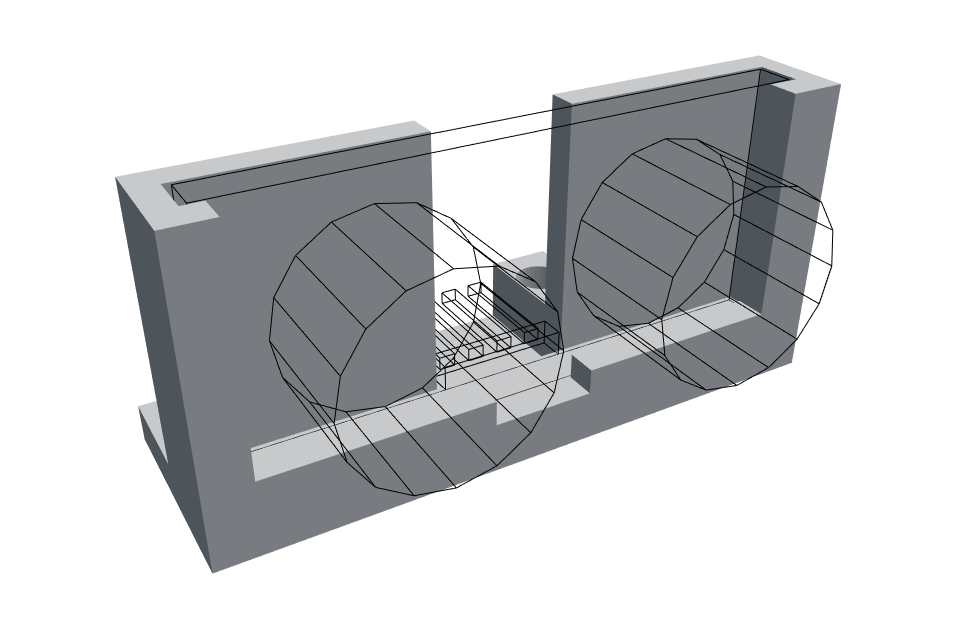
\includegraphics[width=\textwidth]{../3D-Druck_Modelle/Sensorhalterung.png}
	\end{subfigure}%
	\begin{subfigure}{.375\textwidth}
		\centering
		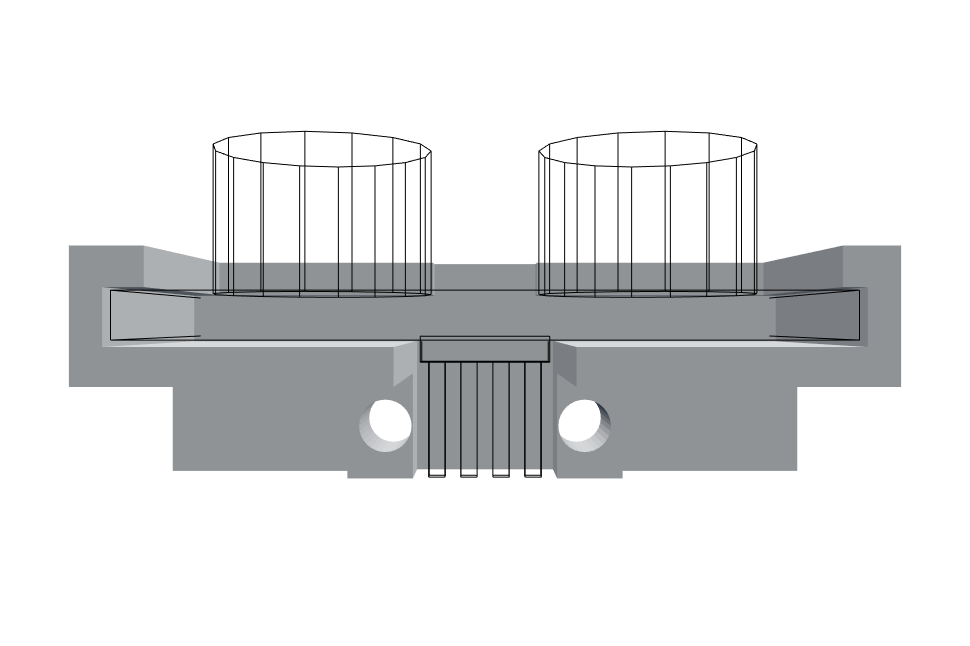
\includegraphics[width=\textwidth]{../3D-Druck_Modelle/Sensorhalterung_Top.png}
	\end{subfigure}\\
	\begin{subfigure}{.375\textwidth}
		\centering
		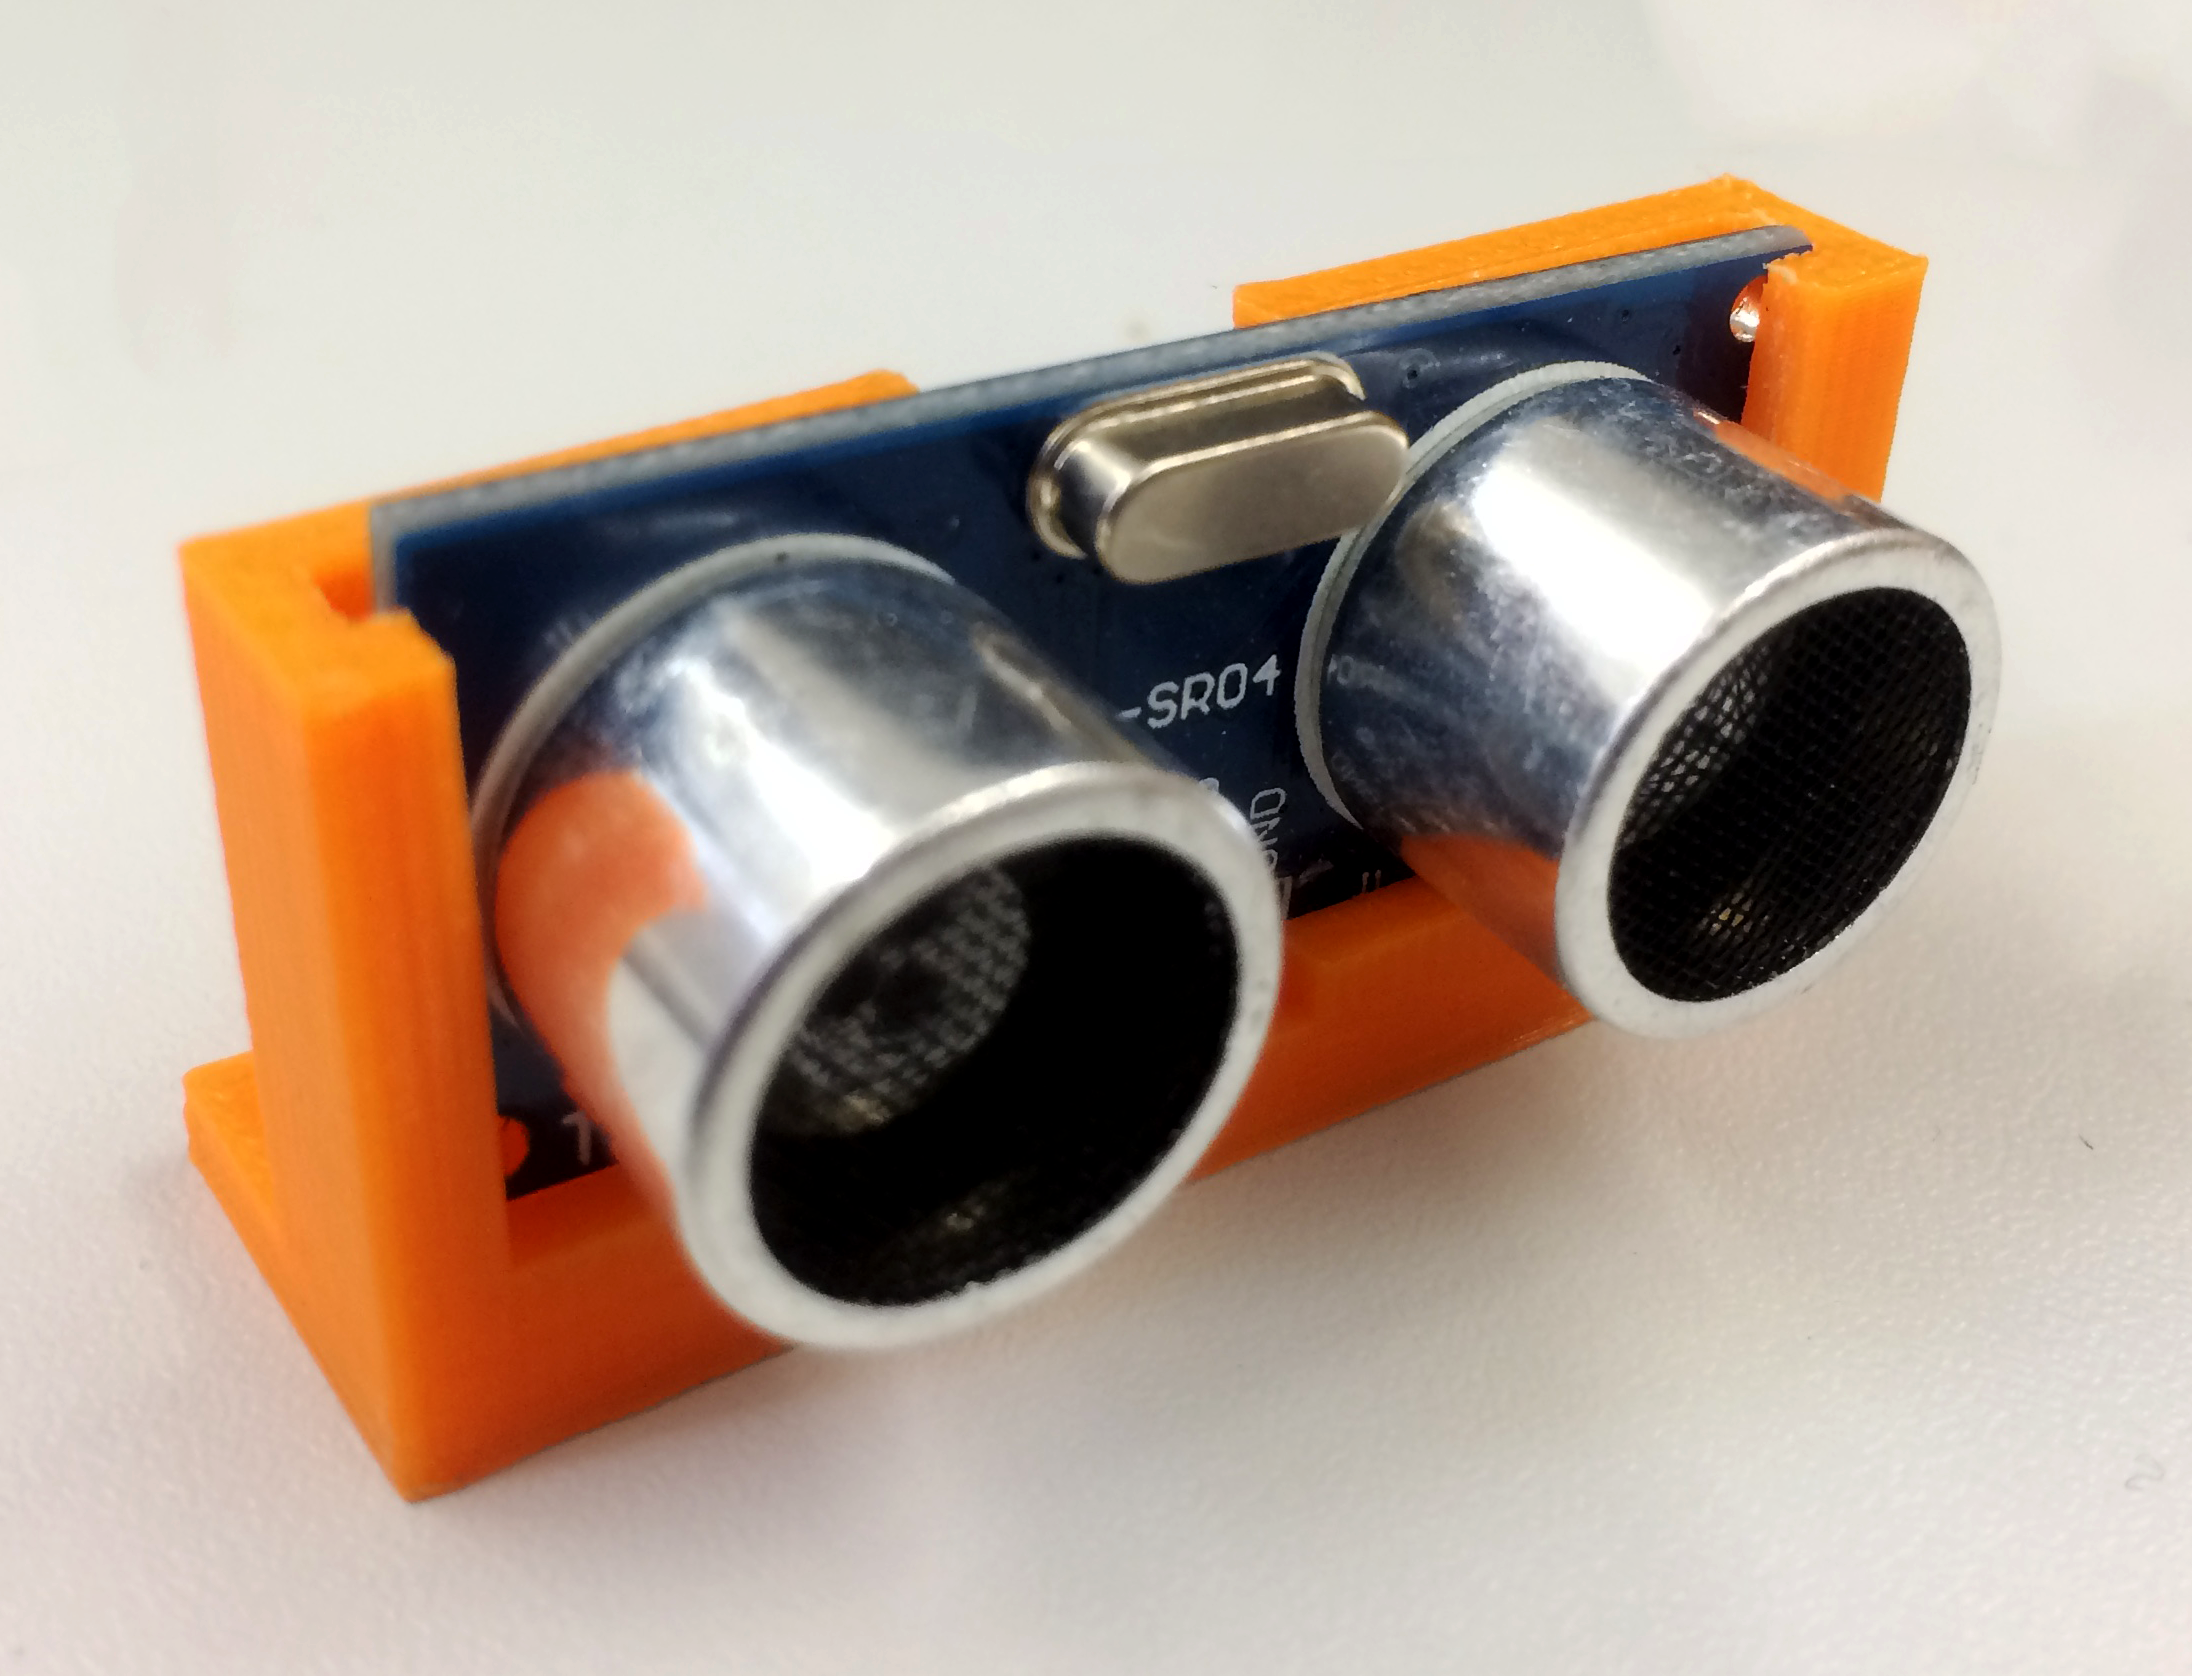
\includegraphics[width=\textwidth]{../bilder_videos/Sensorhalterung.png}
	\end{subfigure}%
	\begin{subfigure}{.375\textwidth}
		\centering
		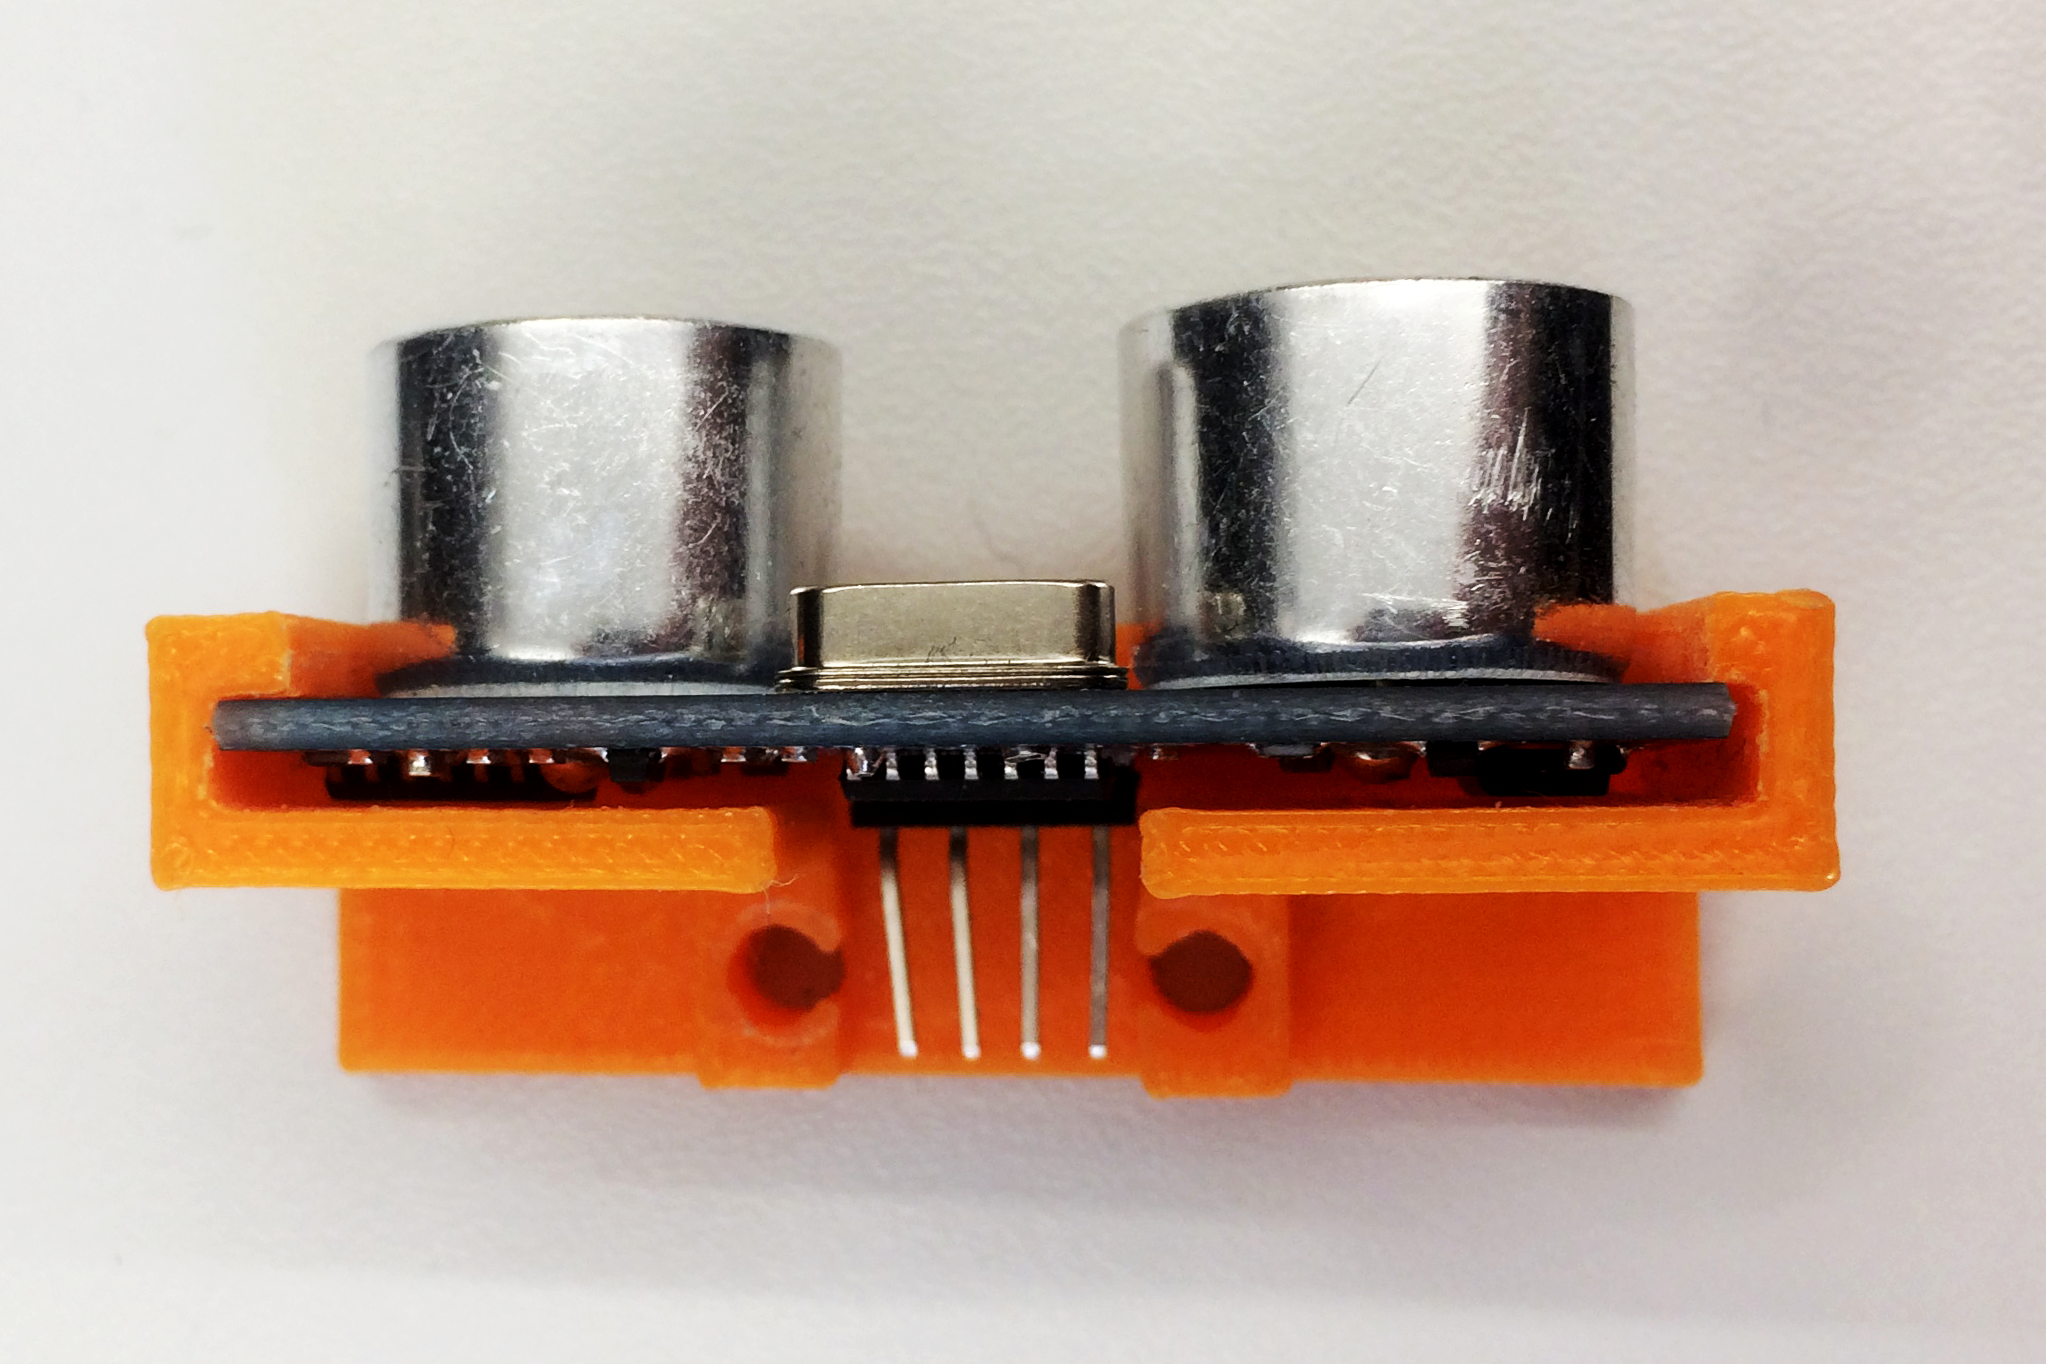
\includegraphics[width=\textwidth]{../bilder_videos/Sensorhalterung_Top.png}
	\end{subfigure}%
	\caption{Ultraschallsensorhalterung 3D-Modell und fertiger 3D-Druck}
\end{figure}

\section{Probleme}
Der günstige Anschaffungspreis des Autobausatzes führte zu einem schnellen Verschleiß der linken Motoren, die wir vor der Prüfung beide austauschen mussten, weil sie durch die fast ausschließlich vorkommenden Rechtskurven stärker beansprucht werden, als die rechten Motoren.

Wie in allen anderen Gruppen machte der Ultraschallsensor nach einiger Zeit Probleme, was allerdings nicht nur auf die minderwertige Qualität zurückzuführen ist. Meistens waren die gemessenen Abstände zur Wand bei Stillstand des Autos bis auf wenige Abweichungen im Toleranzbereich. Erst bei der Fahrt war die konstante Einhaltung des Abstandes zunächst in vielen Fällen nicht zuverlässig, da die Messwerte aus unbekannten Gründen völlig in die Höhe gestiegen sind, obwohl die Distanz nahezu identisch geblieben ist. Dies wurde aber zum Teil durch die Pulsweitenmodulation der Motoren beeinträchtigt, dessen Frequenzen der Rechtecksignale mit dem Senden des Triggers und Empfangen des Echos am Sensor zu Kollisionen führte. Nach einer Anpassung der PWM-Frequenz von \unit[70]{Hz} auf \unit[73]{Hz} funktionierte die Wandfahrt schon deutlich besser und wurde um einiges zuverlässiger. Für zukünftige Projekte wäre es ratsam, auf hochwertigere Ultraschallsensoren umzusteigen und einen Aufpreis in Kauf zu nehmen, aber dafür ein stabileres Fahrverhalten zu gewährleisten.

\section{Ergebnis}

Am Tag der Präsentation konnten wir unsere persönliche Bestzeit vom Vortag nochmals um 15 Sekunden verbessern. Pro Runde benötigte unser Auto durchschnittlich 52 Sekunden, also insgesamt 1:44 Minuten für zwei Runden. Die gesamte Strecke wurde völlig autonom bewältigt, denn unser Auto fuhr problemlos bei der grünen Ampel los und beendete seine Fahrt kurz hinter der Ziellinie nach zwei Runden durch die blaue Ampel. Während der Fahrt befand sich das Auto zu jeder Zeit innerhalb der schwarzen Begrenzungslinien und musste an keiner Stelle neu auf die Strecke gesetzt werden.

\begin{figure}[H]
	\centering
	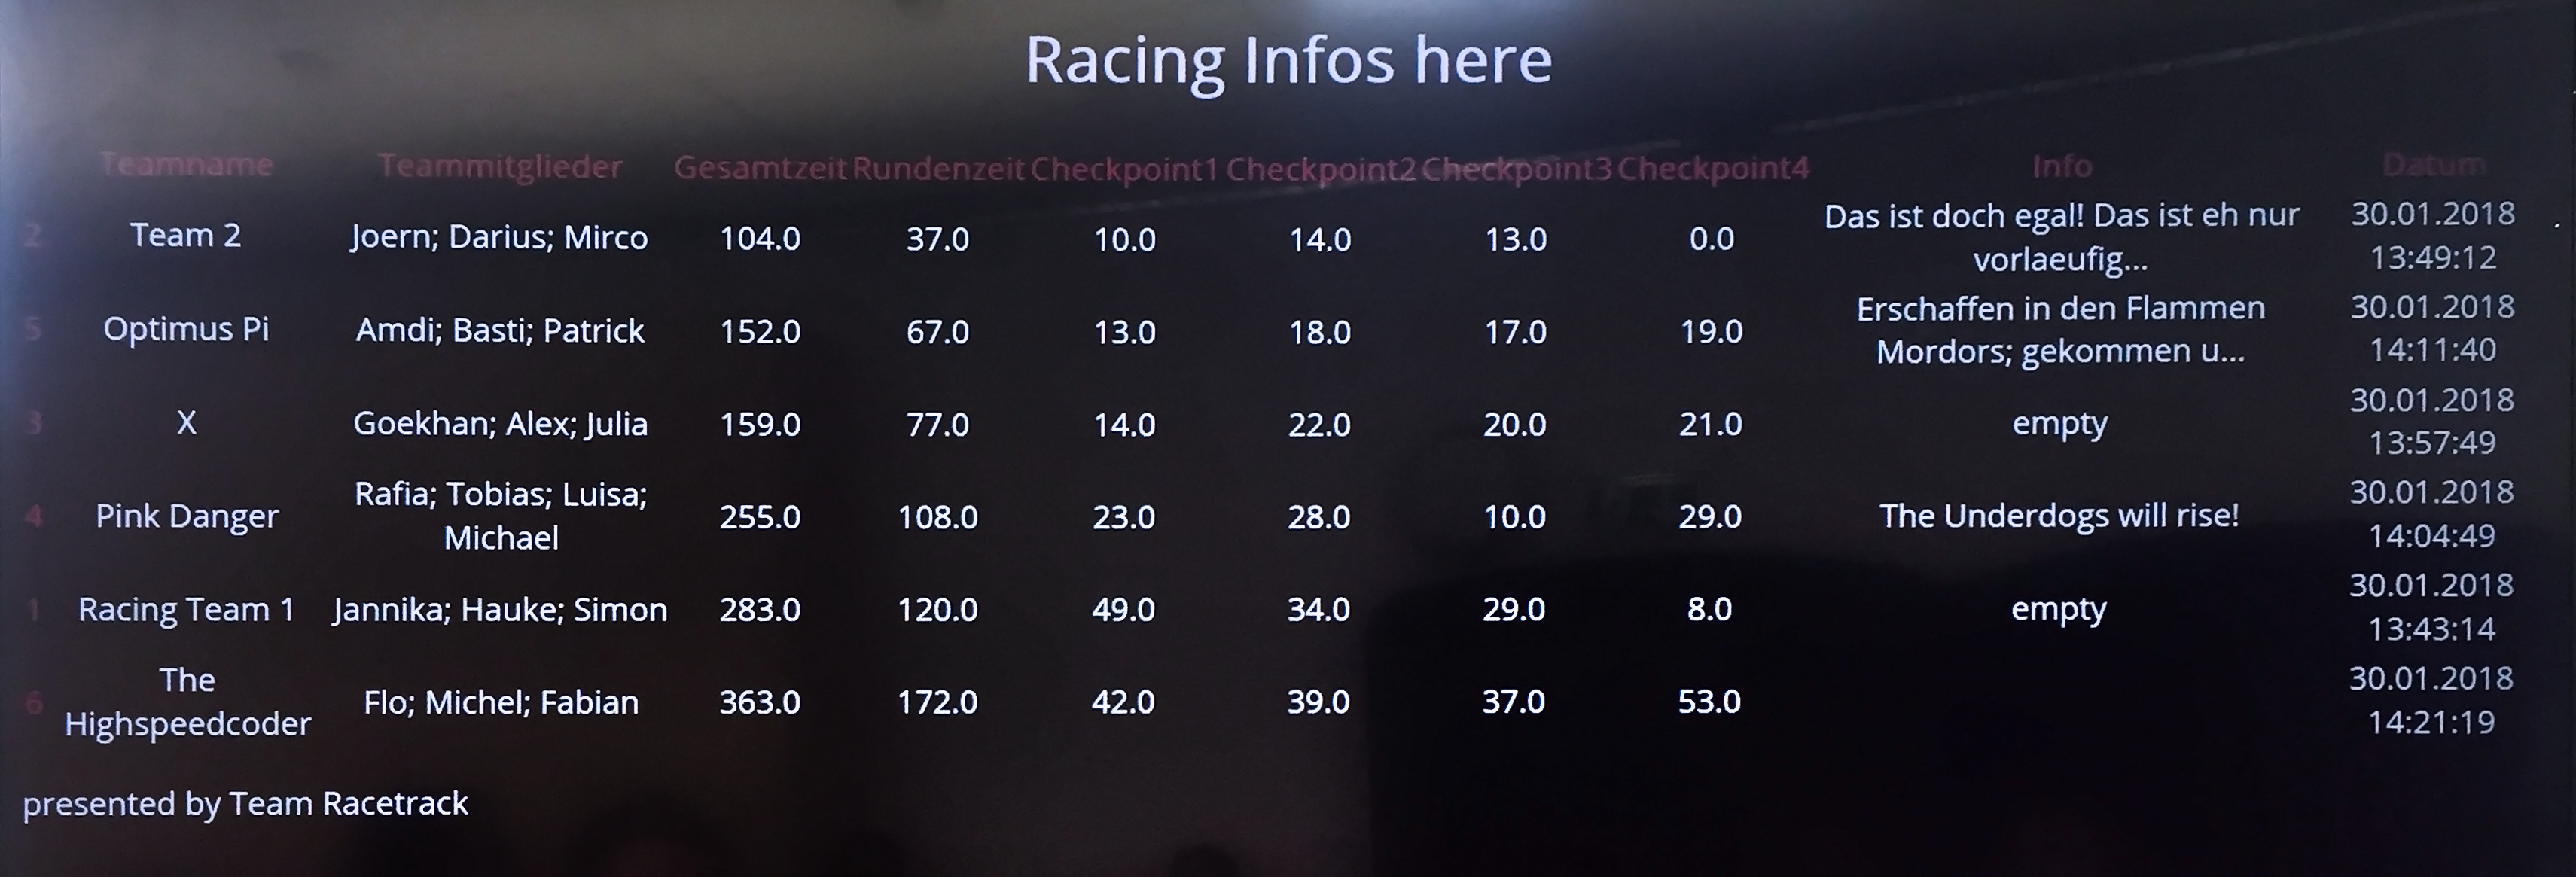
\includegraphics[width=1\textwidth]{Racing_Infos.jpeg}
	\caption{Gesamtzeiten aller ITS-Gruppen}
\end{figure}


Der Abstand von 48 Sekunden zum zweitschnellsten Team ist dadurch zu erklären, dass die Motoren an keiner Stelle mit weniger als \unit[40]{\%} der Höchstgeschwindigkeit betrieben wurden und das Auto selbst in den engsten Kurven immer noch sehr zügig der Linie gefolgt ist, ohne sie dauerhaft zu verlieren und vom Kurs abzukommen. Das Verhältnis zwischen sicherem Fahren und hoher Geschwindigkeit wurde auf dem Raspberry Pi durch unseren Code ideal ausgenutzt.


\section{Geplante Weiterentwicklungen}

Es sind diverse Weiterentwicklungen an dem Auto geplant, die bisher nicht verwirklicht wurden.
Ein Plan ist es, die Videoausgabe deutlich auszubauen. So können mehr Messwerte angezeigt werden, wie zum Beispiel die Lenk- und Geschwindigkeitswerte oder die Drehzahl der Motoren und damit die zurückgelegte Strecke. Optimal wäre die Ausgabe eines Livestreams, was allerdings nur möglich ist, wenn dadurch der Fahralgorithmus nicht verlangsamt wird.
Zudem war eine Anzeige der aktuellen Messwerte über LEDs in Entwicklung.

Der Aufbau der Bauteile auf dem Auto soll noch kompakter werden, indem platzsparender gelötet wird. Dadurch wären alle Platinen auf der unteren Platte platziert, sodass nur noch der Raspberry Pi, der Akku und die Kamera zu sehen sind.

Es ist auch eine andere Herangehensweise an die Programmierung mithilfe von neuronalen Netzen denkbar. So würde das Auto mit der Zeit selbstständig lernen, wie es die Rennstrecke zu absolvieren hat und wie Schwierigkeiten, zum Beispiel enge Kurven, am besten gehandhabt werden können. Danach wäre es auch möglich, wie im Straßenverkehr vorausschauend zu fahren und mögliche Gefahren und Hindernisse frühzeitig zu entdecken und dagegen vorzugehen. Nichtsdestotrotz werden damit Kenntnisse beim Programmieren vorausgesetzt, die wahrscheinlich nicht vollständig innerhalb eines Semesters erlernt werden können.

\newpage

%Tabellenverzeichnis
\listoftables
\addcontentsline{toc}{section}{Tabellenverzeichnis} 

%Abbildungsverzeichnis
\listoffigures
\addcontentsline{toc}{section}{Abbildungsverzeichnis} 

%Literaturverzeichnis
\renewcaptionname{ngerman}{\refname}{Literaturverzeichnis}
\addcontentsline{toc}{section}{Literaturverzeichnis} 

\begin{thebibliography}{}
	\bibitem{}
	Edeler, Torsten: \textit{IT-Systeme}, HAW Hamburg, 13. Oktober 2017
\end{thebibliography}
\end{document}